\begin{frame}[t,label=case-t1-001]{基线的选择影响衰减时间}{T1 Visibility / 001}
\setlength{\parskip}{0pt}
\begingroup
\setlength{\topsep}{0pt}\setlength{\partopsep}{0pt}
\begin{figure}
\centering
{\small
\makebox[.49\linewidth][c]{\textcolor{Teal}{左：基线选择下的时间常数较接近}}%
\makebox[.49\linewidth][c]{\textcolor{Orange}{右：改变基线后时间常数变化}}\par
}
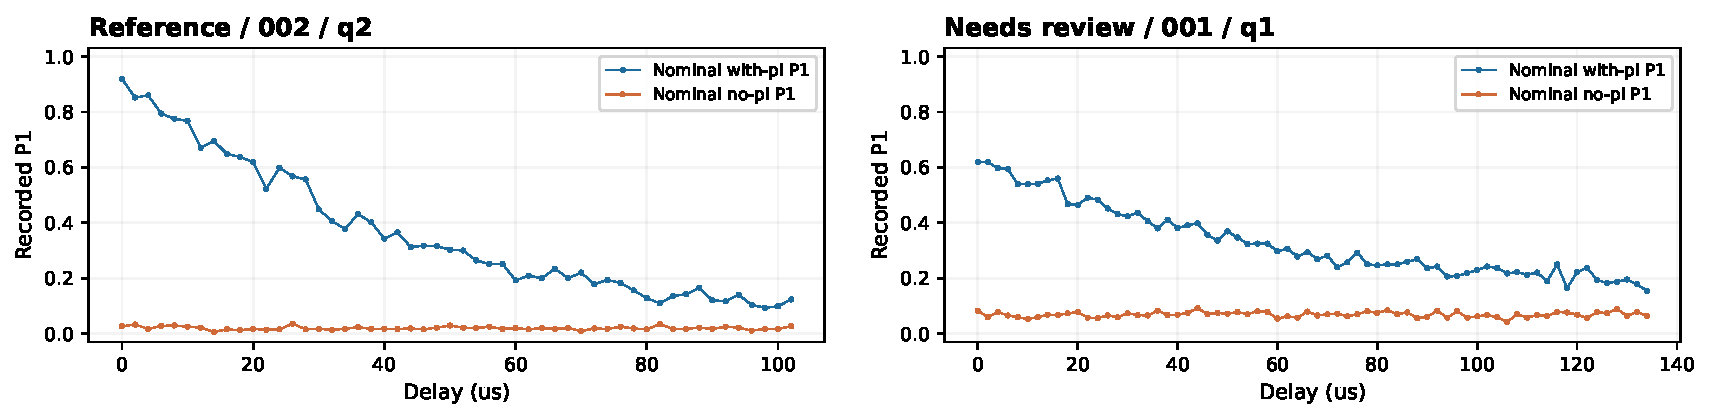
\includegraphics[width=\linewidth,height=34mm,keepaspectratio]{figures/t1-001.pdf}
\caption{左：对照 002；右：案例 001。两路布居差拟合： $\tau_{free}=55.94$ / $\tau_0=77.48\,\mu s$。准备顺序为推断；拟合对象是两路布居差。}
\label{fig-t1-001}
\end{figure}
\endgroup
{\small\textbf{判断：衰减时间依赖基线假设；需延长等待并检查参考通道。}\par}
\end{frame}

\begin{frame}[t,label=case-t1-005]{基线的选择影响衰减时间}{T1 Visibility / 005}
\setlength{\parskip}{0pt}
\begingroup
\setlength{\topsep}{0pt}\setlength{\partopsep}{0pt}
\begin{figure}
\centering
{\small
\makebox[.49\linewidth][c]{\textcolor{Teal}{左：基线选择下的时间常数较接近}}%
\makebox[.49\linewidth][c]{\textcolor{Orange}{右：改变基线后时间常数变化}}\par
}
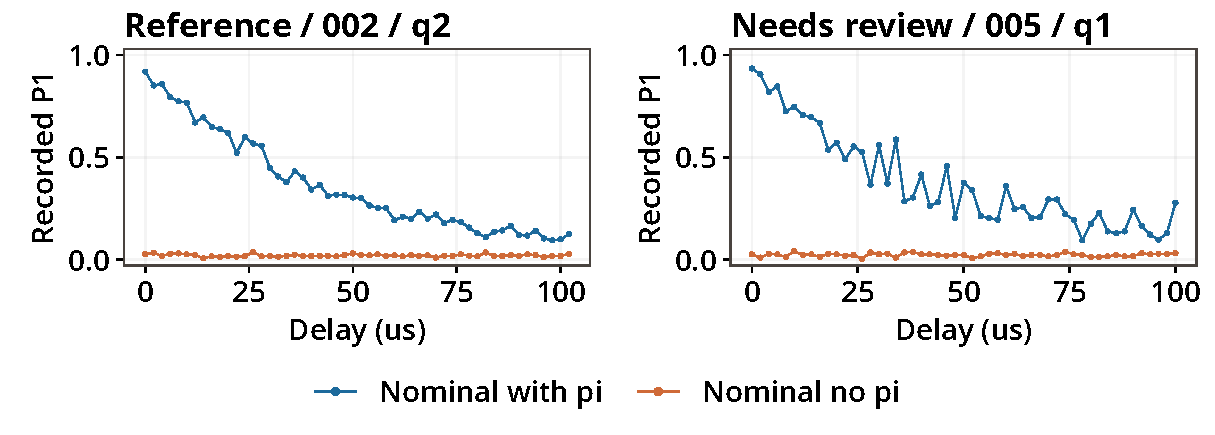
\includegraphics[width=\linewidth,height=34mm,keepaspectratio]{figures/t1-005.pdf}
\caption{左：对照 002；右：案例 005。两路布居差拟合： $\tau_{free}=33.01$ / $\tau_0=44.48\,\mu s$。准备顺序为推断；拟合对象是两路布居差。}
\label{fig-t1-005}
\end{figure}
\endgroup
{\small\textbf{判断：衰减时间依赖基线假设；需延长等待并检查参考通道。}\par}
\end{frame}

\begin{frame}[t,label=case-ramsey-001]{单一包络仍有未解释的结构}{T2 Ramsey / 001}
\setlength{\parskip}{0pt}
\begingroup
\setlength{\topsep}{0pt}\setlength{\partopsep}{0pt}
\begin{figure}
\centering
{\small
\makebox[.49\linewidth][c]{\textcolor{Teal}{左：较清晰的振荡也有相关残差}}%
\makebox[.49\linewidth][c]{\textcolor{Orange}{右：当前模型对记录的解释不足}}\par
}
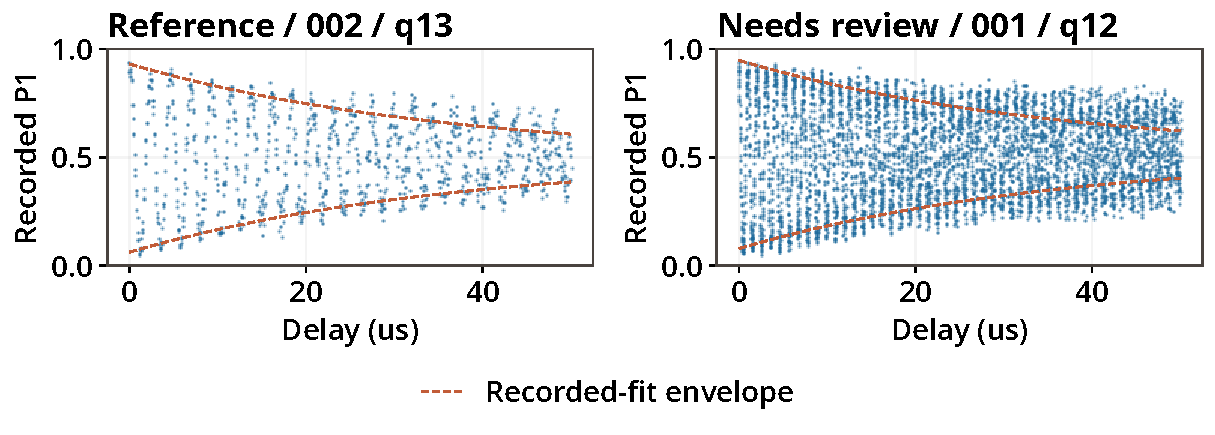
\includegraphics[width=\linewidth,height=34mm,keepaspectratio]{figures/ramsey-001.pdf}
\caption{左：对照 002；右：案例 001。已有拟合： $R^2=0.769$；相邻残差相关系数 $0.10$。对照也有复查项；虚线仅表示包络，不是完整振荡预测。}
\label{fig-ramsey-001}
\end{figure}
\endgroup
{\small\textbf{判断：两侧均需复查；需比较拟合窗口与重复记录，不能只采纳时间常数。}\par}
\end{frame}

\begin{frame}[t,label=case-ramsey-002]{较清晰振荡也留下相关残差}{T2 Ramsey / 002}
\setlength{\parskip}{0pt}
\begingroup
\setlength{\topsep}{0pt}\setlength{\partopsep}{0pt}
\begin{figure}
\centering
{\small
\makebox[.49\linewidth][c]{\textcolor{Teal}{左：较清晰的振荡也有相关残差}}%
\makebox[.49\linewidth][c]{\textcolor{Orange}{右：当前模型仍留下相关残差}}\par
}
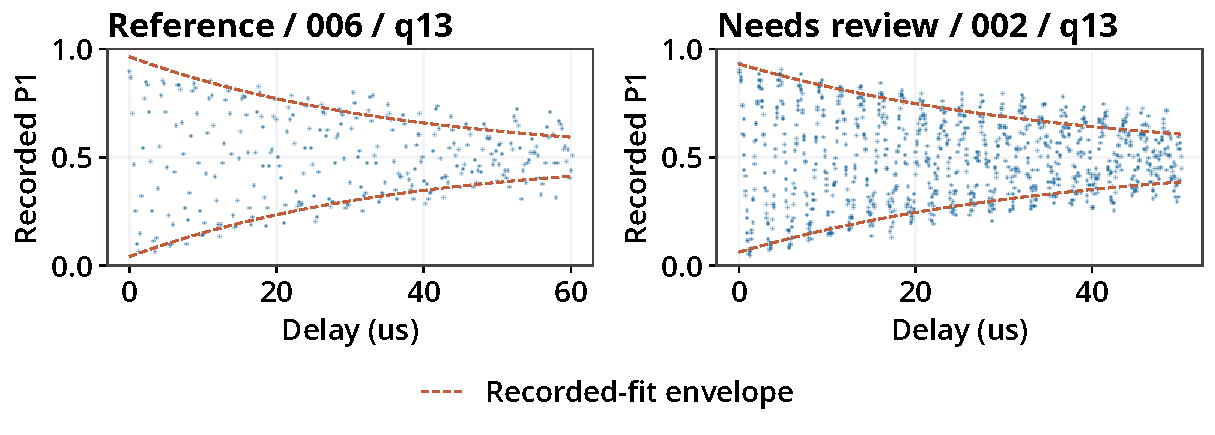
\includegraphics[width=\linewidth,height=34mm,keepaspectratio]{figures/ramsey-002.pdf}
\caption{左：对照 006；右：案例 002。已有拟合： $R^2=0.878$；相邻残差相关系数 $0.32$。对照也有复查项；虚线仅表示包络，不是完整振荡预测。}
\label{fig-ramsey-002}
\end{figure}
\endgroup
{\small\textbf{判断：两侧均需复查；需比较拟合窗口与重复记录，不能只采纳时间常数。}\par}
\end{frame}

\begin{frame}[t,label=case-ramsey-003]{单一包络仍有未解释的结构}{T2 Ramsey / 003}
\setlength{\parskip}{0pt}
\begingroup
\setlength{\topsep}{0pt}\setlength{\partopsep}{0pt}
\begin{figure}
\centering
{\small
\makebox[.49\linewidth][c]{\textcolor{Teal}{左：较清晰的振荡也有相关残差}}%
\makebox[.49\linewidth][c]{\textcolor{Orange}{右：当前模型仍留下相关残差}}\par
}
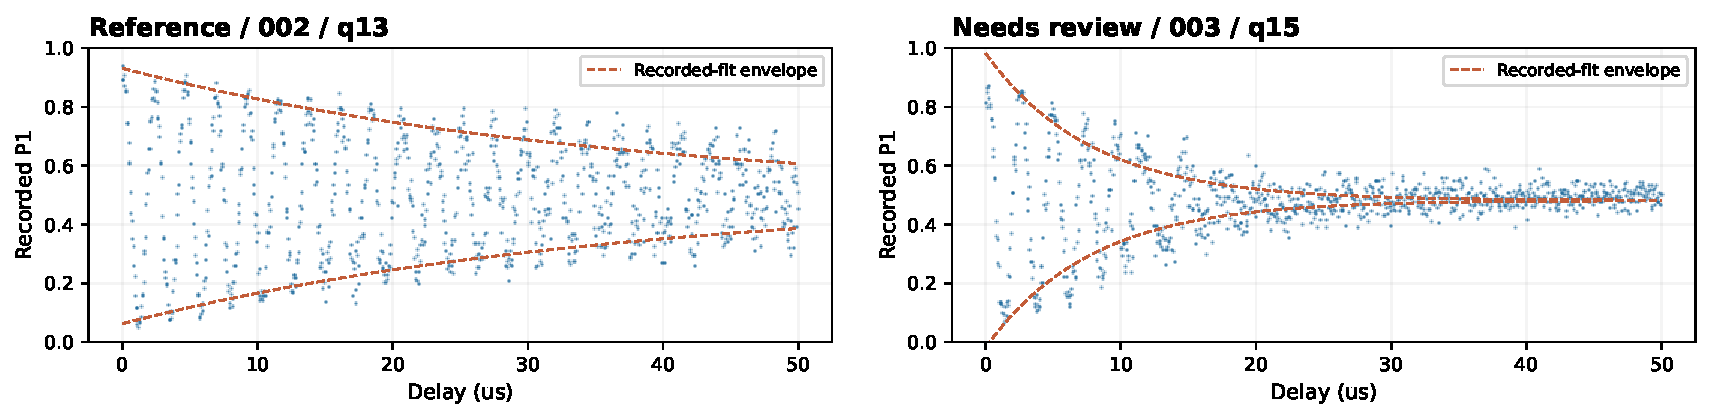
\includegraphics[width=\linewidth,height=34mm,keepaspectratio]{figures/ramsey-003.pdf}
\caption{左：对照 002；右：案例 003。已有拟合： $R^2=0.700$；相邻残差相关系数 $0.48$。对照也有复查项；虚线仅表示包络，不是完整振荡预测。}
\label{fig-ramsey-003}
\end{figure}
\endgroup
{\small\textbf{判断：两侧均需复查；需比较拟合窗口与重复记录，不能只采纳时间常数。}\par}
\end{frame}

\begin{frame}[t,label=case-ramsey-004]{单一包络仍有未解释的结构}{T2 Ramsey / 004}
\setlength{\parskip}{0pt}
\begingroup
\setlength{\topsep}{0pt}\setlength{\partopsep}{0pt}
\begin{figure}
\centering
{\small
\makebox[.49\linewidth][c]{\textcolor{Teal}{左：较清晰的振荡也有相关残差}}%
\makebox[.49\linewidth][c]{\textcolor{Orange}{右：当前模型对记录的解释不足}}\par
}
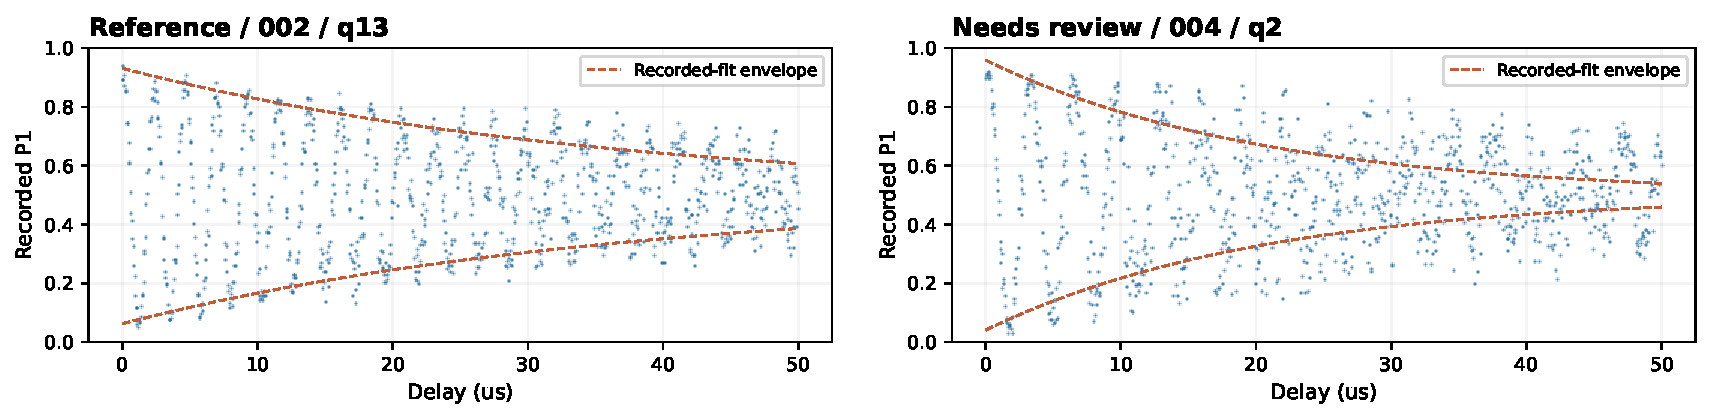
\includegraphics[width=\linewidth,height=34mm,keepaspectratio]{figures/ramsey-004.pdf}
\caption{左：对照 002；右：案例 004。已有拟合： $R^2=0.580$；相邻残差相关系数 $0.22$。对照也有复查项；虚线仅表示包络，不是完整振荡预测。}
\label{fig-ramsey-004}
\end{figure}
\endgroup
{\small\textbf{判断：两侧均需复查；需比较拟合窗口与重复记录，不能只采纳时间常数。}\par}
\end{frame}

\begin{frame}[t,label=case-ramsey-005]{单一包络仍有未解释的结构}{T2 Ramsey / 005}
\setlength{\parskip}{0pt}
\begingroup
\setlength{\topsep}{0pt}\setlength{\partopsep}{0pt}
\begin{figure}
\centering
{\small
\makebox[.49\linewidth][c]{\textcolor{Teal}{左：较清晰的振荡也有相关残差}}%
\makebox[.49\linewidth][c]{\textcolor{Orange}{右：当前模型对记录的解释不足}}\par
}
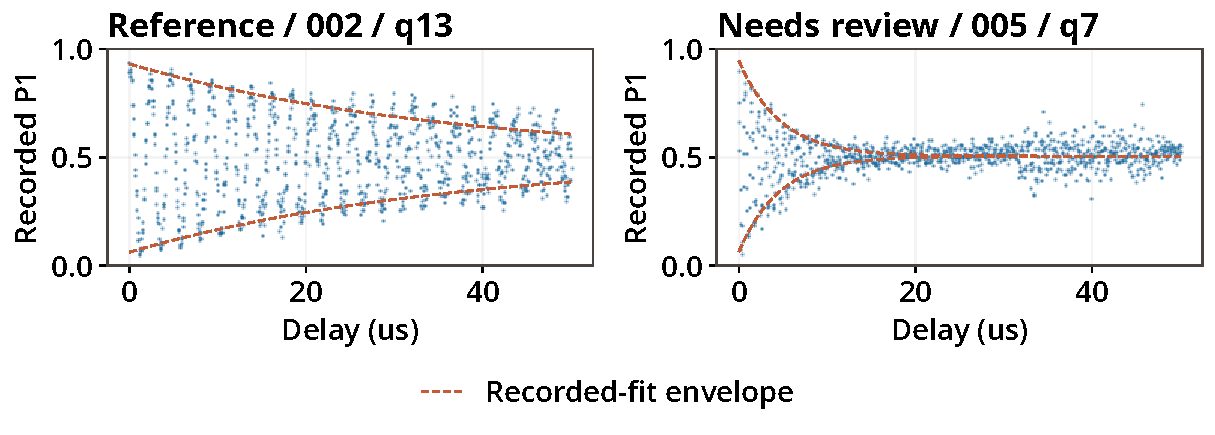
\includegraphics[width=\linewidth,height=34mm,keepaspectratio]{figures/ramsey-005.pdf}
\caption{左：对照 002；右：案例 005。已有拟合： $R^2=0.642$；相邻残差相关系数 $0.17$。对照也有复查项；虚线仅表示包络，不是完整振荡预测。}
\label{fig-ramsey-005}
\end{figure}
\endgroup
{\small\textbf{判断：两侧均需复查；需比较拟合窗口与重复记录，不能只采纳时间常数。}\par}
\end{frame}

\begin{frame}[t,label=case-ramsey-006]{较清晰振荡也留下相关残差}{T2 Ramsey / 006}
\setlength{\parskip}{0pt}
\begingroup
\setlength{\topsep}{0pt}\setlength{\partopsep}{0pt}
\begin{figure}
\centering
{\small
\makebox[.49\linewidth][c]{\textcolor{Teal}{左：较清晰的振荡也有相关残差}}%
\makebox[.49\linewidth][c]{\textcolor{Orange}{右：当前模型仍留下相关残差}}\par
}
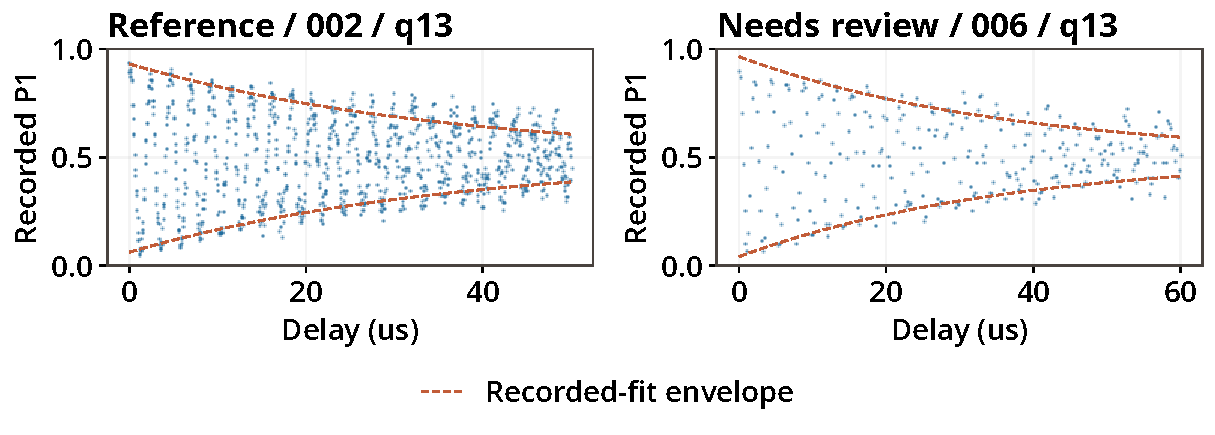
\includegraphics[width=\linewidth,height=34mm,keepaspectratio]{figures/ramsey-006.pdf}
\caption{左：对照 002；右：案例 006。已有拟合： $R^2=0.878$；相邻残差相关系数 $0.37$。对照也有复查项；虚线仅表示包络，不是完整振荡预测。}
\label{fig-ramsey-006}
\end{figure}
\endgroup
{\small\textbf{判断：两侧均需复查；需比较拟合窗口与重复记录，不能只采纳时间常数。}\par}
\end{frame}

\begin{frame}[t,label=case-ramsey-007]{单一包络仍有未解释的结构}{T2 Ramsey / 007}
\setlength{\parskip}{0pt}
\begingroup
\setlength{\topsep}{0pt}\setlength{\partopsep}{0pt}
\begin{figure}
\centering
{\small
\makebox[.49\linewidth][c]{\textcolor{Teal}{左：较清晰的振荡也有相关残差}}%
\makebox[.49\linewidth][c]{\textcolor{Orange}{右：当前模型仍留下相关残差}}\par
}
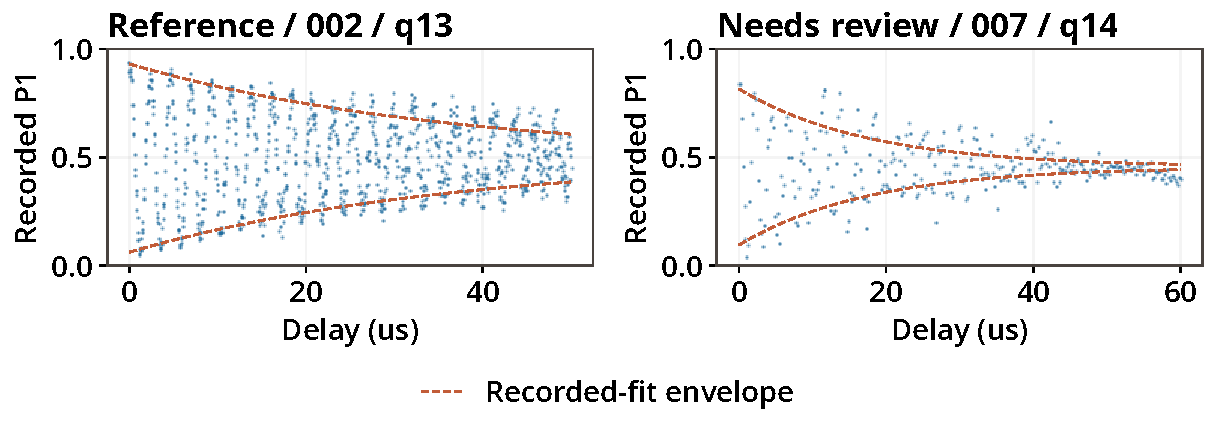
\includegraphics[width=\linewidth,height=34mm,keepaspectratio]{figures/ramsey-007.pdf}
\caption{左：对照 002；右：案例 007。已有拟合： $R^2=0.563$；相邻残差相关系数 $0.37$。对照也有复查项；虚线仅表示包络，不是完整振荡预测。}
\label{fig-ramsey-007}
\end{figure}
\endgroup
{\small\textbf{判断：两侧均需复查；需比较拟合窗口与重复记录，不能只采纳时间常数。}\par}
\end{frame}

\begin{frame}[t,label=case-rabi-001]{噪声状曲线也会返回拟合周期}{Rabi Oscillation / 001}
\setlength{\parskip}{0pt}
\begingroup
\setlength{\topsep}{0pt}\setlength{\partopsep}{0pt}
\begin{figure}
\centering
{\small
\makebox[.49\linewidth][c]{\textcolor{Teal}{左：转折与回返约束一个完整周期}}%
\makebox[.49\linewidth][c]{\textcolor{Orange}{右：散点不支持拟合的快速振荡}}\par
}
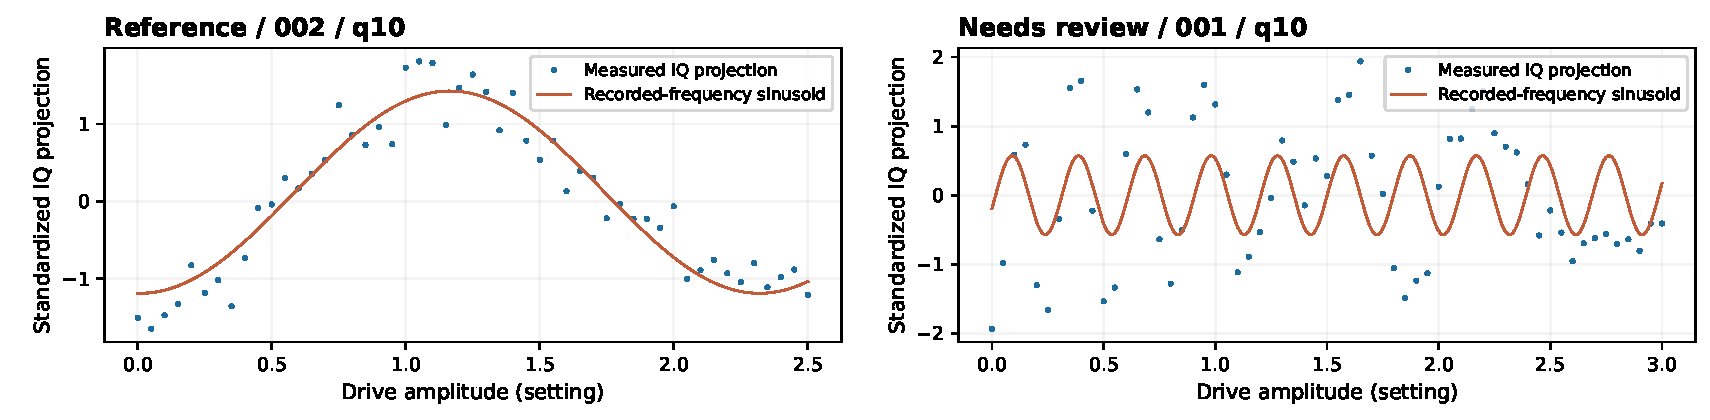
\includegraphics[width=\linewidth,height=34mm,keepaspectratio]{figures/rabi-001.pdf}
\caption{左：对照 002；右：案例 001。IQ 投影拟合： $R^2=0.160$；扫描覆盖 $10.10$ 个周期；每周期 $5.94$ 个采样点。IQ 投影独立标准化，符号与大小不可跨案例比较。}
\label{fig-rabi-001}
\end{figure}
\endgroup
{\small\textbf{判断：不能采用拟合半周期作为 $\pi$ 脉冲设置；需先恢复清晰振荡。}\par}
\end{frame}

\begin{frame}[t,label=case-rabi-004]{单一正弦模型仍有未解释的结构}{Rabi Oscillation / 004}
\setlength{\parskip}{0pt}
\begingroup
\setlength{\topsep}{0pt}\setlength{\partopsep}{0pt}
\begin{figure}
\centering
{\small
\makebox[.49\linewidth][c]{\textcolor{Teal}{左：转折与回返约束一个完整周期}}%
\makebox[.49\linewidth][c]{\textcolor{Orange}{右：正弦拟合仍留下结构性残差}}\par
}
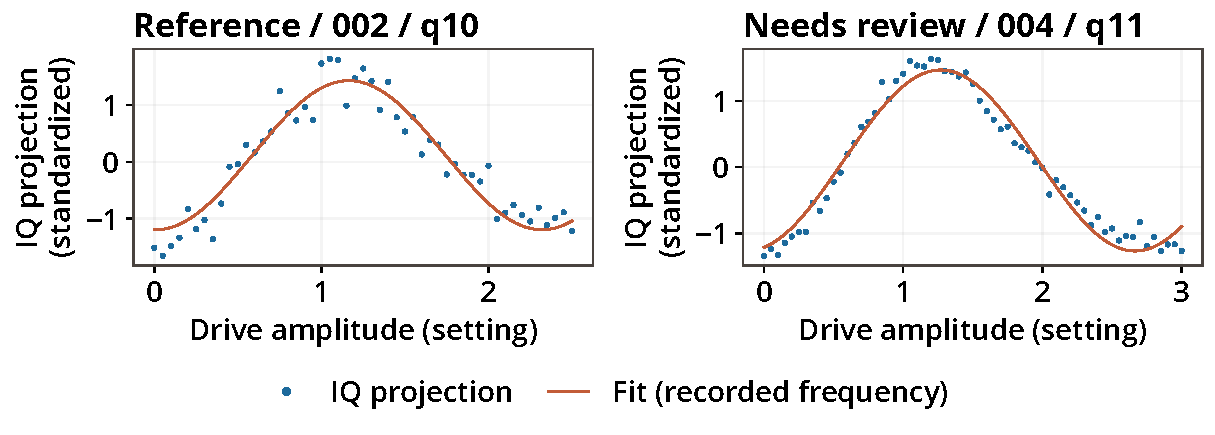
\includegraphics[width=\linewidth,height=34mm,keepaspectratio]{figures/rabi-004.pdf}
\caption{左：对照 002；右：案例 004。IQ 投影拟合： $R^2=0.967$；扫描覆盖 $1.08$ 个周期。IQ 投影独立标准化，符号与大小不可跨案例比较。}
\label{fig-rabi-004}
\end{figure}
\endgroup
{\small\textbf{判断：需复测并检查驱动与模型；单一正弦拟合尚不足以确认设置。}\par}
\end{frame}

\begin{frame}[t,label=case-rabi-005]{IQ 分布偏离固定两态连线}{Rabi Oscillation / 005}
\setlength{\parskip}{0pt}
\begingroup
\setlength{\topsep}{0pt}\setlength{\partopsep}{0pt}
\begin{figure}
\centering
{\small
\makebox[.49\linewidth][c]{\textcolor{Teal}{左：转折与回返约束一个完整周期}}%
\makebox[.49\linewidth][c]{\textcolor{Orange}{右：投影拟合未验证两态连线近似}}\par
}
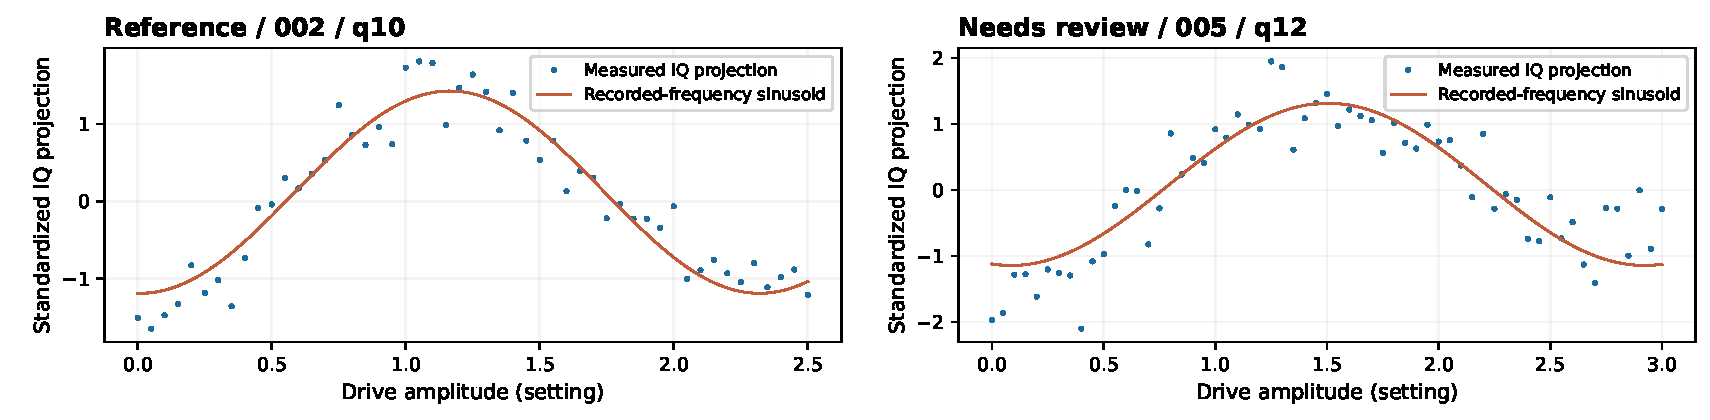
\includegraphics[width=\linewidth,height=34mm,keepaspectratio]{figures/rabi-005.pdf}
\caption{左：对照 002；右：案例 005。IQ 投影拟合： $R^2=0.798$；扫描覆盖 $1.06$ 个周期。IQ 投影独立标准化，符号与大小不可跨案例比较。}
\label{fig-rabi-005}
\end{figure}
\endgroup
{\small\textbf{判断：需检查完整 IQ 轨迹；投影与几何诊断尚不能确定物理原因。}\par}
\end{frame}

\begin{frame}[t,label=case-rabi-006]{IQ 分布偏离固定两态连线}{Rabi Oscillation / 006}
\setlength{\parskip}{0pt}
\begingroup
\setlength{\topsep}{0pt}\setlength{\partopsep}{0pt}
\begin{figure}
\centering
{\small
\makebox[.49\linewidth][c]{\textcolor{Teal}{左：转折与回返约束一个完整周期}}%
\makebox[.49\linewidth][c]{\textcolor{Orange}{右：投影拟合未验证两态连线近似}}\par
}
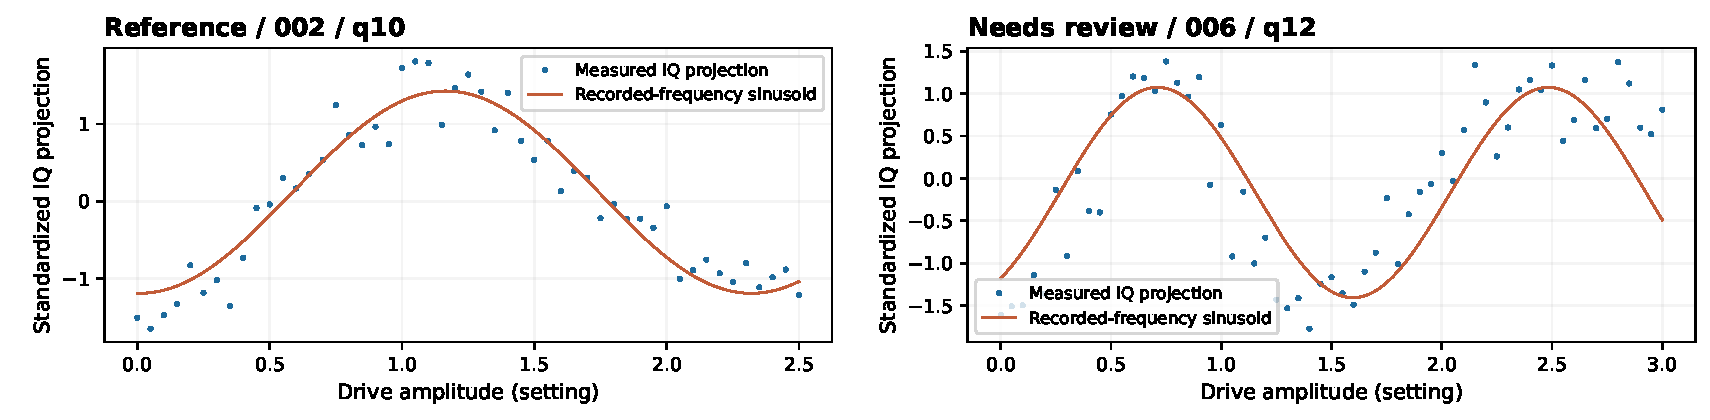
\includegraphics[width=\linewidth,height=34mm,keepaspectratio]{figures/rabi-006.pdf}
\caption{左：对照 002；右：案例 006。IQ 投影拟合： $R^2=0.689$；扫描覆盖 $1.69$ 个周期。IQ 投影独立标准化，符号与大小不可跨案例比较。}
\label{fig-rabi-006}
\end{figure}
\endgroup
{\small\textbf{判断：需检查完整 IQ 轨迹；投影与几何诊断尚不能确定物理原因。}\par}
\end{frame}

\begin{frame}[t,label=case-rabi-008]{局部曲线不足以约束周期}{Rabi Oscillation / 008}
\setlength{\parskip}{0pt}
\begingroup
\setlength{\topsep}{0pt}\setlength{\partopsep}{0pt}
\begin{figure}
\centering
{\small
\makebox[.49\linewidth][c]{\textcolor{Teal}{左：转折与回返约束一个完整周期}}%
\makebox[.49\linewidth][c]{\textcolor{Orange}{右：扫描只覆盖局部曲线}}\par
}
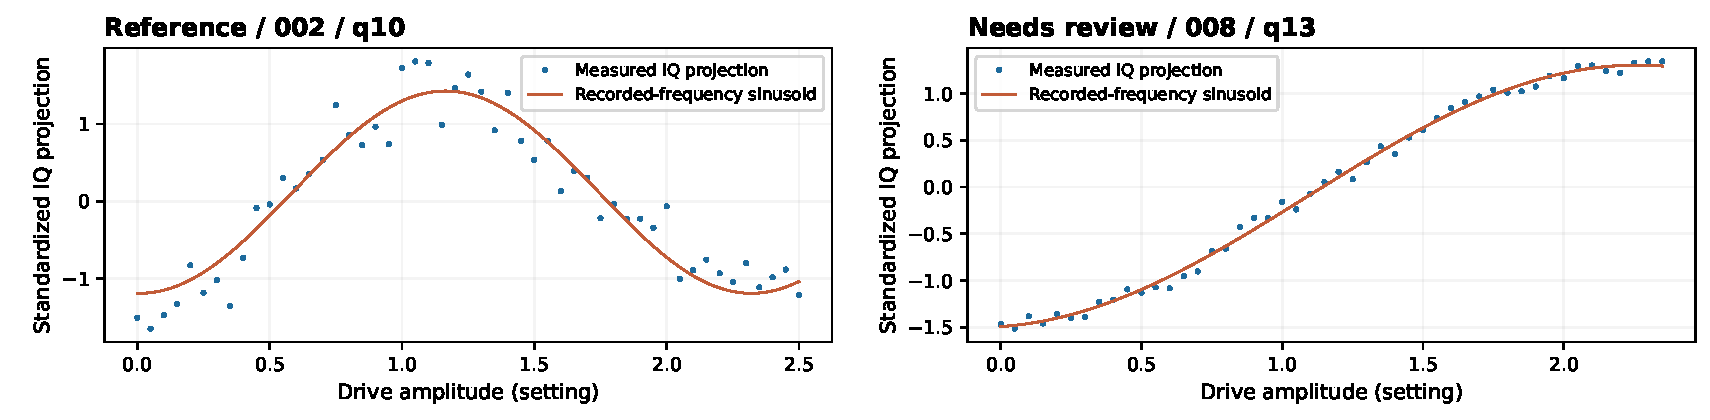
\includegraphics[width=\linewidth,height=34mm,keepaspectratio]{figures/rabi-008.pdf}
\caption{左：对照 002；右：案例 008。IQ 投影拟合： $R^2=0.996$；扫描覆盖 $0.50$ 个周期。IQ 投影独立标准化，符号与大小不可跨案例比较。}
\label{fig-rabi-008}
\end{figure}
\endgroup
{\small\textbf{判断：周期主要依赖外推；需扩大幅度范围，观察转折与回返。}\par}
\end{frame}

\begin{frame}[t,label=case-rabi-009]{单一正弦模型仍有未解释的结构}{Rabi Oscillation / 009}
\setlength{\parskip}{0pt}
\begingroup
\setlength{\topsep}{0pt}\setlength{\partopsep}{0pt}
\begin{figure}
\centering
{\small
\makebox[.49\linewidth][c]{\textcolor{Teal}{左：转折与回返约束一个完整周期}}%
\makebox[.49\linewidth][c]{\textcolor{Orange}{右：正弦拟合仍留下结构性残差}}\par
}
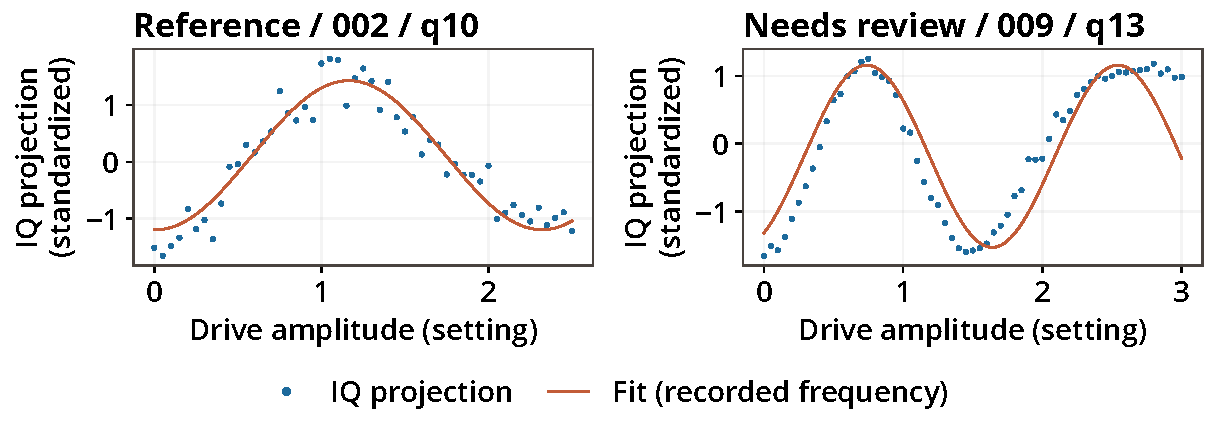
\includegraphics[width=\linewidth,height=34mm,keepaspectratio]{figures/rabi-009.pdf}
\caption{左：对照 002；右：案例 009。IQ 投影拟合： $R^2=0.824$；扫描覆盖 $1.66$ 个周期。IQ 投影独立标准化，符号与大小不可跨案例比较。}
\label{fig-rabi-009}
\end{figure}
\endgroup
{\small\textbf{判断：需复测并检查驱动与模型；单一正弦拟合尚不足以确认设置。}\par}
\end{frame}

\begin{frame}[t,label=case-rabi-010]{单一正弦模型仍有未解释的结构}{Rabi Oscillation / 010}
\setlength{\parskip}{0pt}
\begingroup
\setlength{\topsep}{0pt}\setlength{\partopsep}{0pt}
\begin{figure}
\centering
{\small
\makebox[.49\linewidth][c]{\textcolor{Teal}{左：转折与回返约束一个完整周期}}%
\makebox[.49\linewidth][c]{\textcolor{Orange}{右：正弦拟合仍留下结构性残差}}\par
}
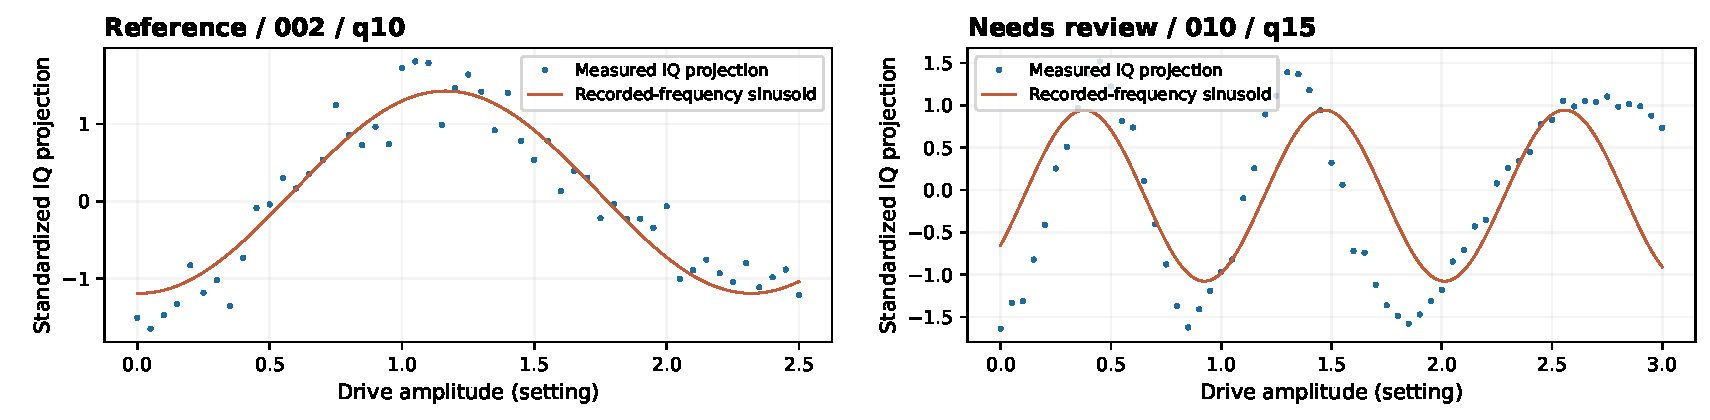
\includegraphics[width=\linewidth,height=34mm,keepaspectratio]{figures/rabi-010.pdf}
\caption{左：对照 002；右：案例 010。IQ 投影拟合： $R^2=0.480$；扫描覆盖 $2.76$ 个周期。IQ 投影独立标准化，符号与大小不可跨案例比较。}
\label{fig-rabi-010}
\end{figure}
\endgroup
{\small\textbf{判断：需复测并检查驱动与模型；单一正弦拟合尚不足以确认设置。}\par}
\end{frame}

\begin{frame}[t,label=case-rabi-011]{单一正弦模型仍有未解释的结构}{Rabi Oscillation / 011}
\setlength{\parskip}{0pt}
\begingroup
\setlength{\topsep}{0pt}\setlength{\partopsep}{0pt}
\begin{figure}
\centering
{\small
\makebox[.49\linewidth][c]{\textcolor{Teal}{左：转折与回返约束一个完整周期}}%
\makebox[.49\linewidth][c]{\textcolor{Orange}{右：正弦拟合仍留下结构性残差}}\par
}
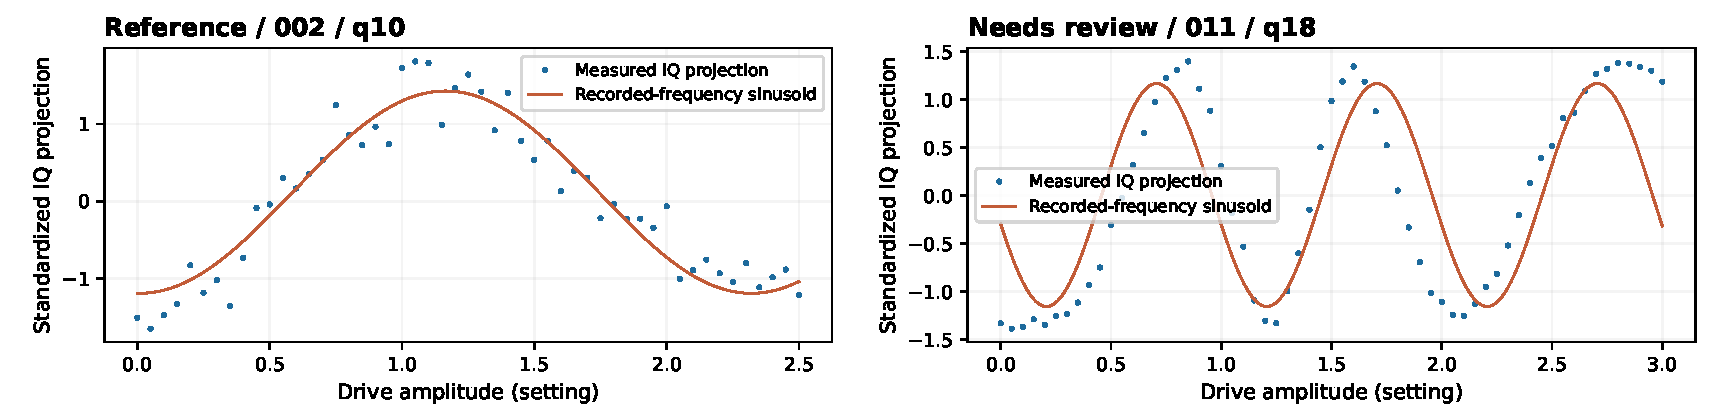
\includegraphics[width=\linewidth,height=34mm,keepaspectratio]{figures/rabi-011.pdf}
\caption{左：对照 002；右：案例 011。IQ 投影拟合： $R^2=0.664$；扫描覆盖 $3.00$ 个周期。IQ 投影独立标准化，符号与大小不可跨案例比较。}
\label{fig-rabi-011}
\end{figure}
\endgroup
{\small\textbf{判断：需复测并检查驱动与模型；单一正弦拟合尚不足以确认设置。}\par}
\end{frame}

\begin{frame}[t,label=case-rabi-012]{单一正弦模型仍有未解释的结构}{Rabi Oscillation / 012}
\setlength{\parskip}{0pt}
\begingroup
\setlength{\topsep}{0pt}\setlength{\partopsep}{0pt}
\begin{figure}
\centering
{\small
\makebox[.49\linewidth][c]{\textcolor{Teal}{左：转折与回返约束一个完整周期}}%
\makebox[.49\linewidth][c]{\textcolor{Orange}{右：正弦拟合仍留下结构性残差}}\par
}
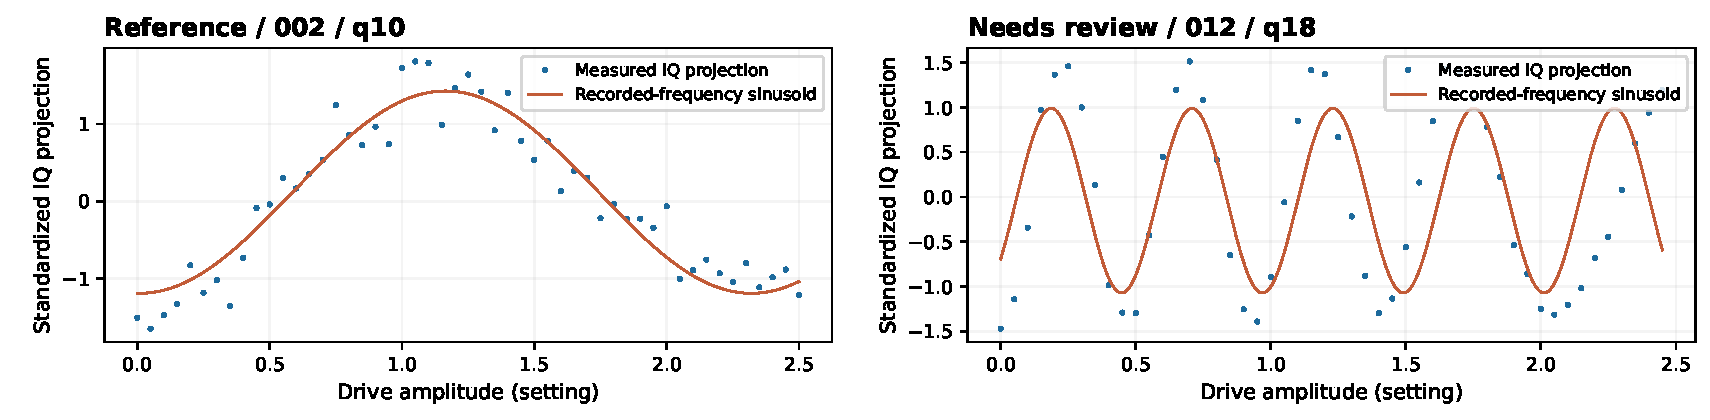
\includegraphics[width=\linewidth,height=34mm,keepaspectratio]{figures/rabi-012.pdf}
\caption{左：对照 002；右：案例 012。IQ 投影拟合： $R^2=0.512$；扫描覆盖 $4.70$ 个周期。IQ 投影独立标准化，符号与大小不可跨案例比较。}
\label{fig-rabi-012}
\end{figure}
\endgroup
{\small\textbf{判断：需复测并检查驱动与模型；单一正弦拟合尚不足以确认设置。}\par}
\end{frame}

\begin{frame}[t,label=case-rabi-013]{单一正弦模型仍有未解释的结构}{Rabi Oscillation / 013}
\setlength{\parskip}{0pt}
\begingroup
\setlength{\topsep}{0pt}\setlength{\partopsep}{0pt}
\begin{figure}
\centering
{\small
\makebox[.49\linewidth][c]{\textcolor{Teal}{左：转折与回返约束一个完整周期}}%
\makebox[.49\linewidth][c]{\textcolor{Orange}{右：正弦拟合仍留下结构性残差}}\par
}
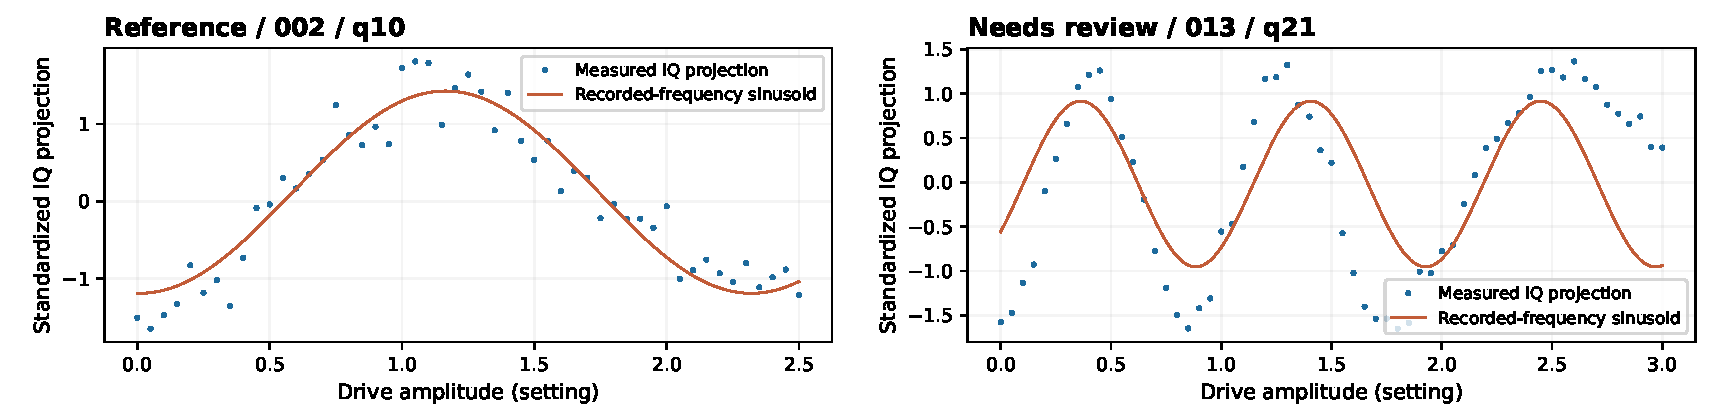
\includegraphics[width=\linewidth,height=34mm,keepaspectratio]{figures/rabi-013.pdf}
\caption{左：对照 002；右：案例 013。IQ 投影拟合： $R^2=0.432$；扫描覆盖 $2.88$ 个周期。IQ 投影独立标准化，符号与大小不可跨案例比较。}
\label{fig-rabi-013}
\end{figure}
\endgroup
{\small\textbf{判断：需复测并检查驱动与模型；单一正弦拟合尚不足以确认设置。}\par}
\end{frame}

\begin{frame}[t,label=case-rabi-014]{单一正弦模型仍有未解释的结构}{Rabi Oscillation / 014}
\setlength{\parskip}{0pt}
\begingroup
\setlength{\topsep}{0pt}\setlength{\partopsep}{0pt}
\begin{figure}
\centering
{\small
\makebox[.49\linewidth][c]{\textcolor{Teal}{左：转折与回返约束一个完整周期}}%
\makebox[.49\linewidth][c]{\textcolor{Orange}{右：正弦拟合仍留下结构性残差}}\par
}
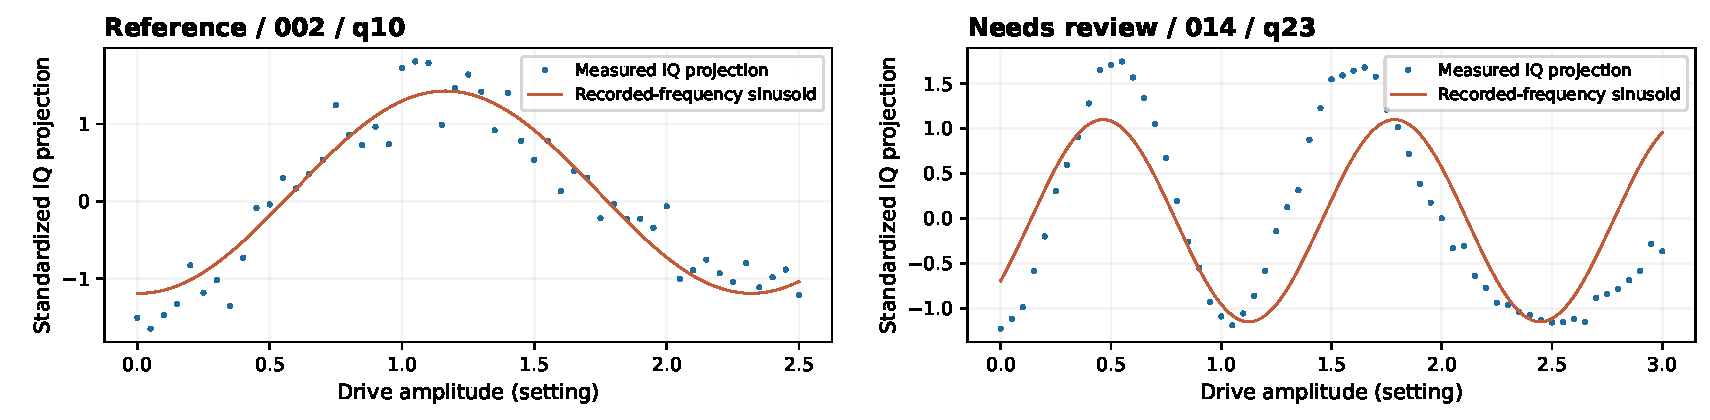
\includegraphics[width=\linewidth,height=34mm,keepaspectratio]{figures/rabi-014.pdf}
\caption{左：对照 002；右：案例 014。IQ 投影拟合： $R^2=0.594$；扫描覆盖 $2.27$ 个周期。IQ 投影独立标准化，符号与大小不可跨案例比较。}
\label{fig-rabi-014}
\end{figure}
\endgroup
{\small\textbf{判断：需复测并检查驱动与模型；单一正弦拟合尚不足以确认设置。}\par}
\end{frame}

\begin{frame}[t,label=case-rabi-015]{局部曲线不足以约束周期}{Rabi Oscillation / 015}
\setlength{\parskip}{0pt}
\begingroup
\setlength{\topsep}{0pt}\setlength{\partopsep}{0pt}
\begin{figure}
\centering
{\small
\makebox[.49\linewidth][c]{\textcolor{Teal}{左：转折与回返约束一个完整周期}}%
\makebox[.49\linewidth][c]{\textcolor{Orange}{右：扫描只覆盖局部曲线}}\par
}
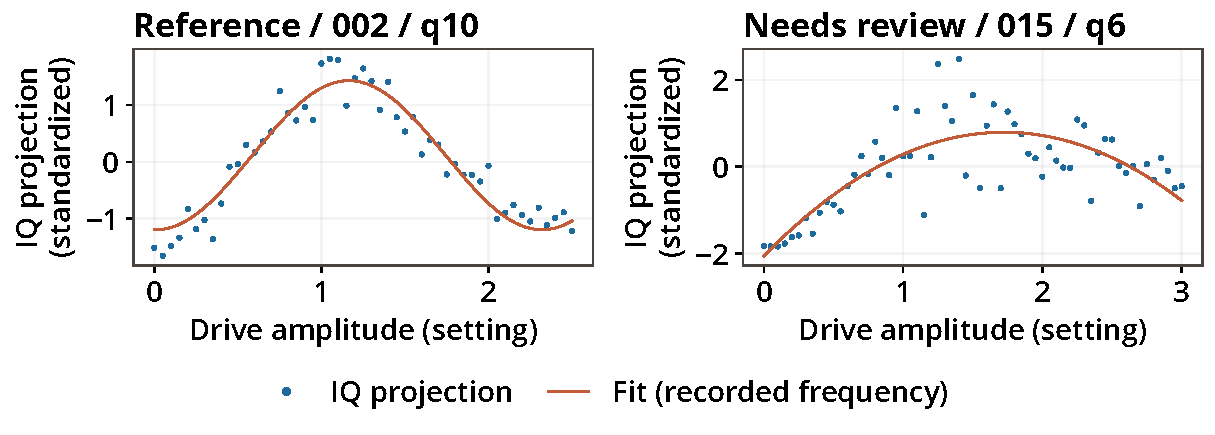
\includegraphics[width=\linewidth,height=34mm,keepaspectratio]{figures/rabi-015.pdf}
\caption{左：对照 002；右：案例 015。IQ 投影拟合： $R^2=0.586$；扫描覆盖 $0.10$ 个周期。IQ 投影独立标准化，符号与大小不可跨案例比较。}
\label{fig-rabi-015}
\end{figure}
\endgroup
{\small\textbf{判断：周期主要依赖外推；需扩大幅度范围，观察转折与回返。}\par}
\end{frame}

\begin{frame}[t,label=case-rabi-016]{单一正弦模型仍有未解释的结构}{Rabi Oscillation / 016}
\setlength{\parskip}{0pt}
\begingroup
\setlength{\topsep}{0pt}\setlength{\partopsep}{0pt}
\begin{figure}
\centering
{\small
\makebox[.49\linewidth][c]{\textcolor{Teal}{左：转折与回返约束一个完整周期}}%
\makebox[.49\linewidth][c]{\textcolor{Orange}{右：正弦拟合仍留下结构性残差}}\par
}
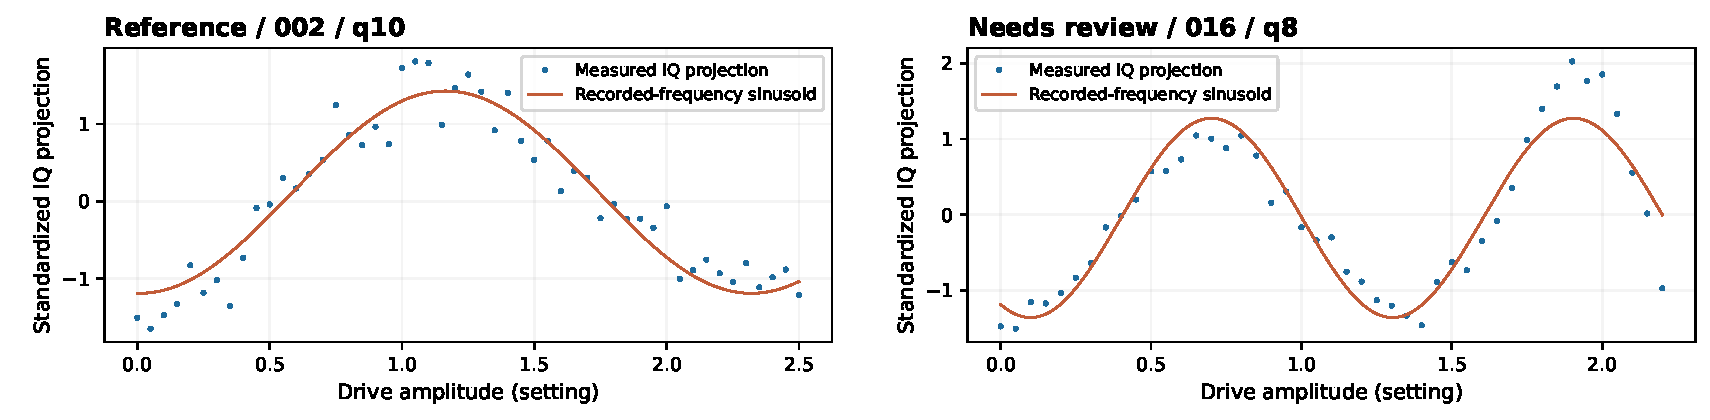
\includegraphics[width=\linewidth,height=34mm,keepaspectratio]{figures/rabi-016.pdf}
\caption{左：对照 002；右：案例 016。IQ 投影拟合： $R^2=0.894$；扫描覆盖 $1.83$ 个周期。IQ 投影独立标准化，符号与大小不可跨案例比较。}
\label{fig-rabi-016}
\end{figure}
\endgroup
{\small\textbf{判断：需复测并检查驱动与模型；单一正弦拟合尚不足以确认设置。}\par}
\end{frame}

\begin{frame}[t,label=case-spectroscopy-002]{背景中的候选响应仍需验证}{Qubit Spectroscopy / 002}
\setlength{\parskip}{0pt}
\begingroup
\setlength{\topsep}{0pt}\setlength{\partopsep}{0pt}
\begin{figure}
\centering
{\small
\makebox[.49\linewidth][c]{\textcolor{Teal}{左：窗口内可见响应与两侧背景}}%
\makebox[.49\linewidth][c]{\textcolor{Orange}{右：背景中的候选响应不够明确}}\par
}
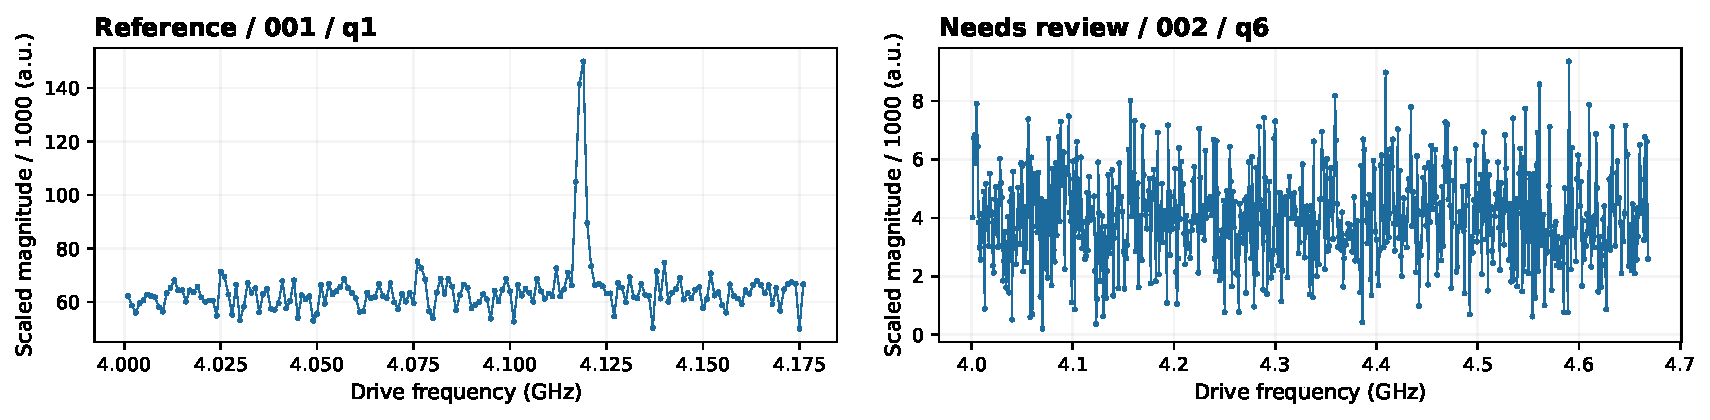
\includegraphics[width=\linewidth,height=34mm,keepaspectratio]{figures/spectroscopy-002.pdf}
\caption{左：对照 001；右：案例 002。IQ 投影诊断： $R^2=0.016$；步长 1.00 / 半高全宽 1.08 MHz。图示幅度；指标来自 IQ 投影的单洛伦兹线形拟合。}
\label{fig-spectroscopy-002}
\end{figure}
\endgroup
{\small\textbf{判断：尚不能确认跃迁频率；需验证信号路径并复测候选响应。}\par}
\end{frame}

\begin{frame}[t,label=case-spectroscopy-004]{可见响应仍需检查线形模型}{Qubit Spectroscopy / 004}
\setlength{\parskip}{0pt}
\begingroup
\setlength{\topsep}{0pt}\setlength{\partopsep}{0pt}
\begin{figure}
\centering
{\small
\makebox[.49\linewidth][c]{\textcolor{Teal}{左：窗口内可见响应与两侧背景}}%
\makebox[.49\linewidth][c]{\textcolor{Orange}{右：单线形拟合仍有未解释结构}}\par
}
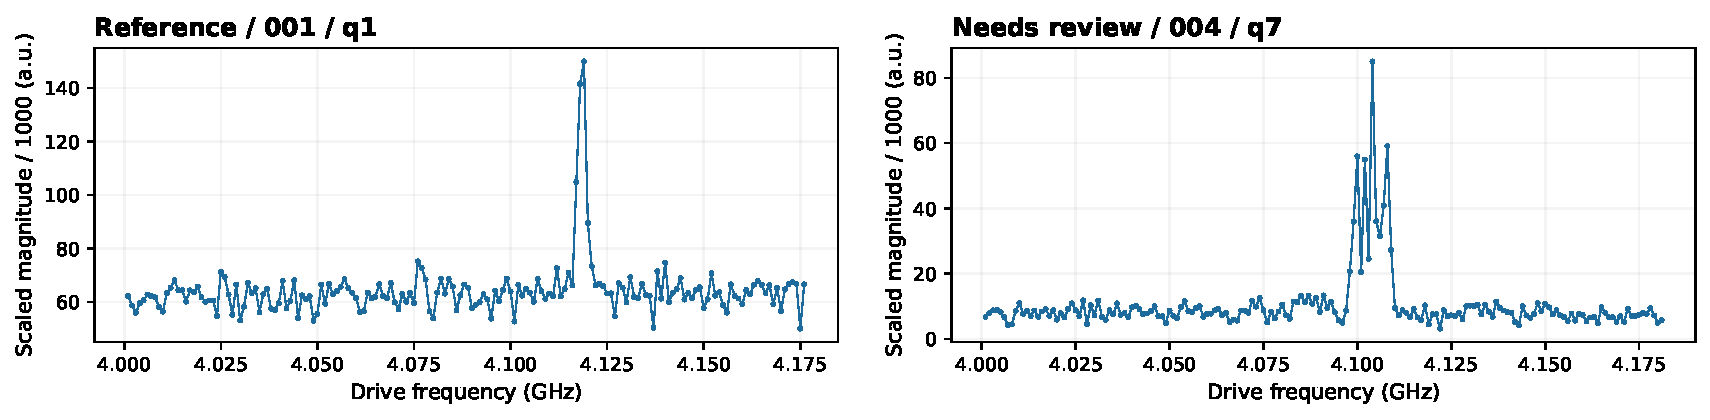
\includegraphics[width=\linewidth,height=34mm,keepaspectratio]{figures/spectroscopy-004.pdf}
\caption{左：对照 001；右：案例 004。IQ 投影诊断： $R^2=0.682$；步长 1.00 / 半高全宽 7.55 MHz。图示幅度；指标来自 IQ 投影的单洛伦兹线形拟合。}
\label{fig-spectroscopy-004}
\end{figure}
\endgroup
{\small\textbf{判断：可见响应不保证单线形模型适用；需细扫并检查线形与背景。}\par}
\end{frame}

\begin{frame}[t,label=case-spectroscopy-006]{可见响应仍需检查线形模型}{Qubit Spectroscopy / 006}
\setlength{\parskip}{0pt}
\begingroup
\setlength{\topsep}{0pt}\setlength{\partopsep}{0pt}
\begin{figure}
\centering
{\small
\makebox[.49\linewidth][c]{\textcolor{Teal}{左：窗口内可见响应与两侧背景}}%
\makebox[.49\linewidth][c]{\textcolor{Orange}{右：单线形拟合仍有未解释结构}}\par
}
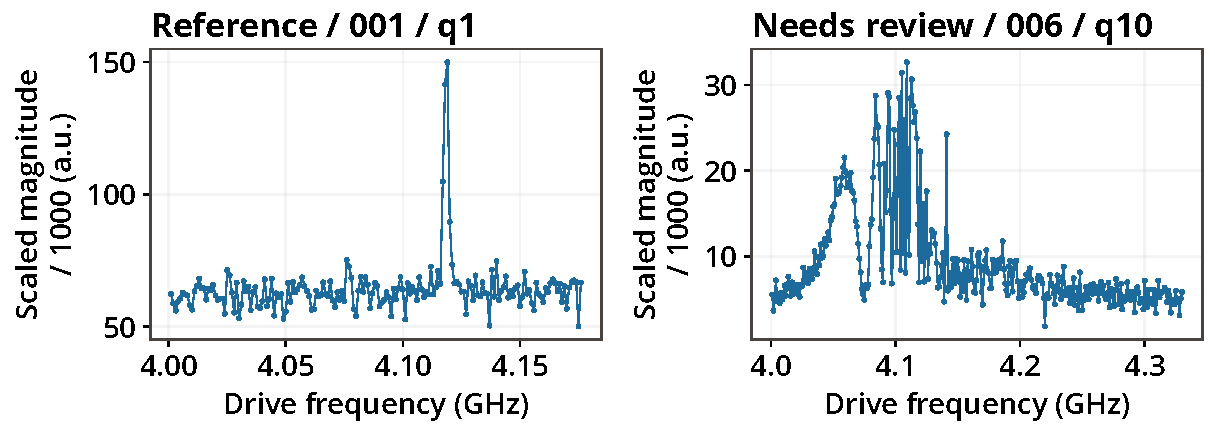
\includegraphics[width=\linewidth,height=34mm,keepaspectratio]{figures/spectroscopy-006.pdf}
\caption{左：对照 001；右：案例 006。IQ 投影诊断： $R^2=0.545$；步长 1.00 / 半高全宽 116.37 MHz。图示幅度；指标来自 IQ 投影的单洛伦兹线形拟合。}
\label{fig-spectroscopy-006}
\end{figure}
\endgroup
{\small\textbf{判断：可见响应不保证单线形模型适用；需细扫并检查线形与背景。}\par}
\end{frame}

\begin{frame}[t,label=case-spectroscopy-007]{频率步长不能分辨拟合线宽}{Qubit Spectroscopy / 007}
\setlength{\parskip}{0pt}
\begingroup
\setlength{\topsep}{0pt}\setlength{\partopsep}{0pt}
\begin{figure}
\centering
{\small
\makebox[.49\linewidth][c]{\textcolor{Teal}{左：窗口内可见响应与两侧背景}}%
\makebox[.49\linewidth][c]{\textcolor{Orange}{右：候选线宽内采样点不足}}\par
}
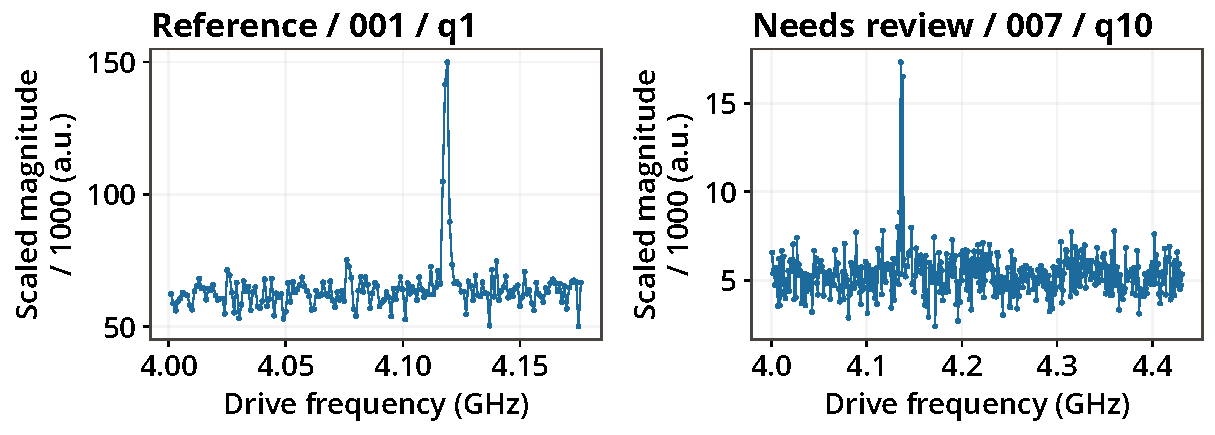
\includegraphics[width=\linewidth,height=34mm,keepaspectratio]{figures/spectroscopy-007.pdf}
\caption{左：对照 001；右：案例 007。IQ 投影诊断： $R^2=0.265$；步长 1.00 / 半高全宽 1.57 MHz。图示幅度；指标来自 IQ 投影的单洛伦兹线形拟合。}
\label{fig-spectroscopy-007}
\end{figure}
\endgroup
{\small\textbf{判断：线宽缺乏采样约束；需局部细扫并复测。}\par}
\end{frame}

\begin{frame}[t,label=case-spectroscopy-009]{频率步长不能分辨拟合线宽}{Qubit Spectroscopy / 009}
\setlength{\parskip}{0pt}
\begingroup
\setlength{\topsep}{0pt}\setlength{\partopsep}{0pt}
\begin{figure}
\centering
{\small
\makebox[.49\linewidth][c]{\textcolor{Teal}{左：窗口内可见响应与两侧背景}}%
\makebox[.49\linewidth][c]{\textcolor{Orange}{右：候选线宽内采样点不足}}\par
}
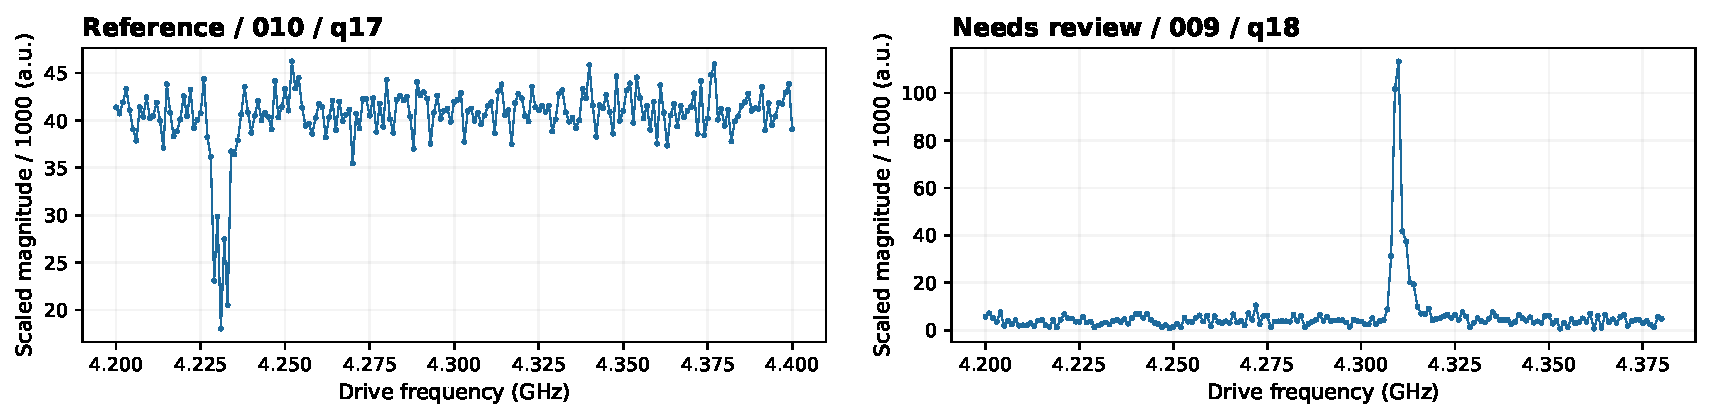
\includegraphics[width=\linewidth,height=34mm,keepaspectratio]{figures/spectroscopy-009.pdf}
\caption{左：对照 010；右：案例 009。IQ 投影诊断： $R^2=0.948$；步长 1.00 / 半高全宽 1.85 MHz。图示幅度；指标来自 IQ 投影的单洛伦兹线形拟合。}
\label{fig-spectroscopy-009}
\end{figure}
\endgroup
{\small\textbf{判断：线宽缺乏采样约束；需局部细扫并复测。}\par}
\end{frame}

\begin{frame}[t,label=case-spectroscopy-011]{背景中的候选响应仍需验证}{Qubit Spectroscopy / 011}
\setlength{\parskip}{0pt}
\begingroup
\setlength{\topsep}{0pt}\setlength{\partopsep}{0pt}
\begin{figure}
\centering
{\small
\makebox[.49\linewidth][c]{\textcolor{Teal}{左：窗口内可见响应与两侧背景}}%
\makebox[.49\linewidth][c]{\textcolor{Orange}{右：背景中的候选响应不够明确}}\par
}
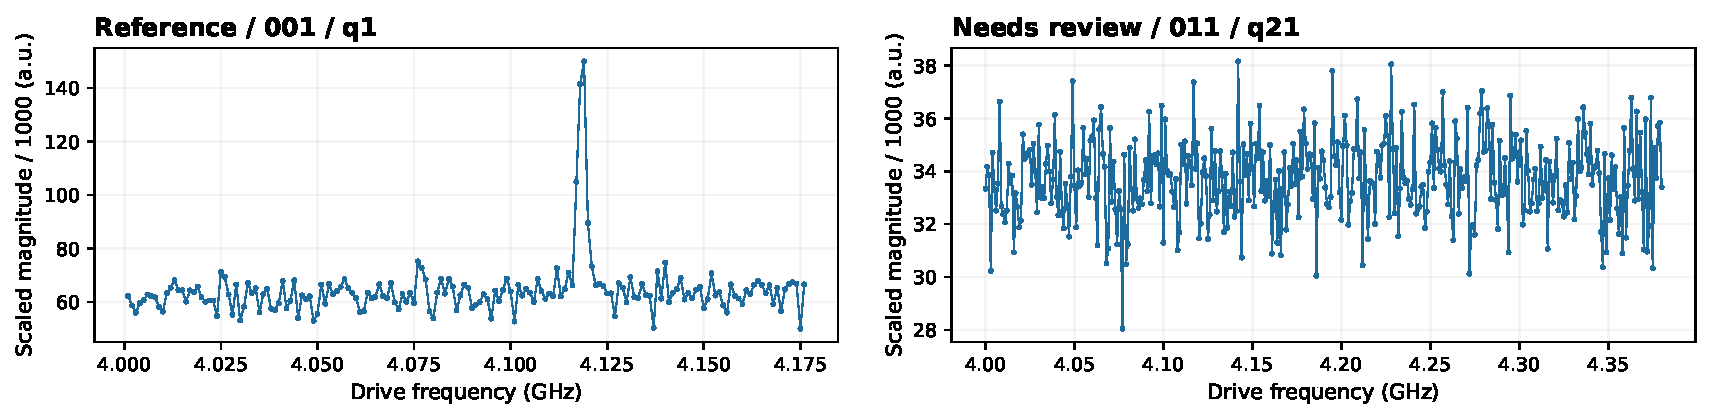
\includegraphics[width=\linewidth,height=34mm,keepaspectratio]{figures/spectroscopy-011.pdf}
\caption{左：对照 001；右：案例 011。IQ 投影诊断： $R^2=0.044$；步长 1.00 / 半高全宽 2.11 MHz。图示幅度；指标来自 IQ 投影的单洛伦兹线形拟合。}
\label{fig-spectroscopy-011}
\end{figure}
\endgroup
{\small\textbf{判断：尚不能确认跃迁频率；需验证信号路径并复测候选响应。}\par}
\end{frame}

\begin{frame}[t,label=case-spectroscopy-012]{扫描边界限制了中心频率的判断}{Qubit Spectroscopy / 012}
\setlength{\parskip}{0pt}
\begingroup
\setlength{\topsep}{0pt}\setlength{\partopsep}{0pt}
\begin{figure}
\centering
{\small
\makebox[.49\linewidth][c]{\textcolor{Teal}{左：窗口内可见响应与两侧背景}}%
\makebox[.49\linewidth][c]{\textcolor{Orange}{右：边缘响应未被完整覆盖}}\par
}
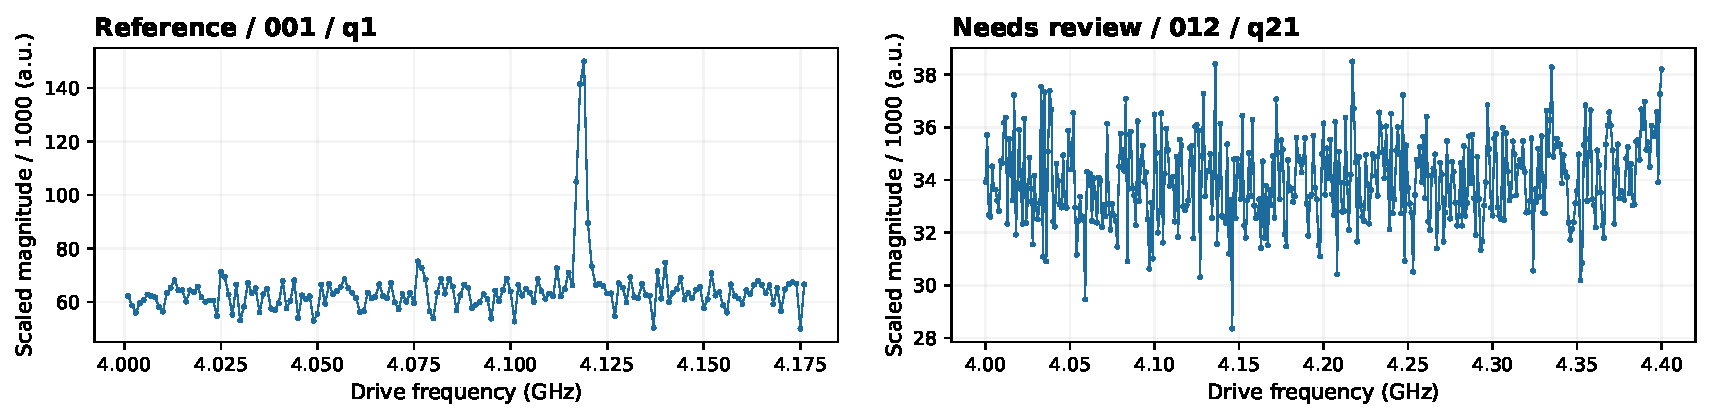
\includegraphics[width=\linewidth,height=34mm,keepaspectratio]{figures/spectroscopy-012.pdf}
\caption{左：对照 001；右：案例 012。IQ 投影诊断： $R^2=0.065$；步长 1.00 / 半高全宽 782.41 MHz。图示幅度；指标来自 IQ 投影的单洛伦兹线形拟合。}
\label{fig-spectroscopy-012}
\end{figure}
\endgroup
{\small\textbf{判断：中心频率缺乏两侧数据约束；需扩大扫描窗口。}\par}
\end{frame}

\begin{frame}[t,label=case-spectroscopy-013]{可见响应仍需检查线形模型}{Qubit Spectroscopy / 013}
\setlength{\parskip}{0pt}
\begingroup
\setlength{\topsep}{0pt}\setlength{\partopsep}{0pt}
\begin{figure}
\centering
{\small
\makebox[.49\linewidth][c]{\textcolor{Teal}{左：窗口内可见响应与两侧背景}}%
\makebox[.49\linewidth][c]{\textcolor{Orange}{右：单线形拟合仍有未解释结构}}\par
}
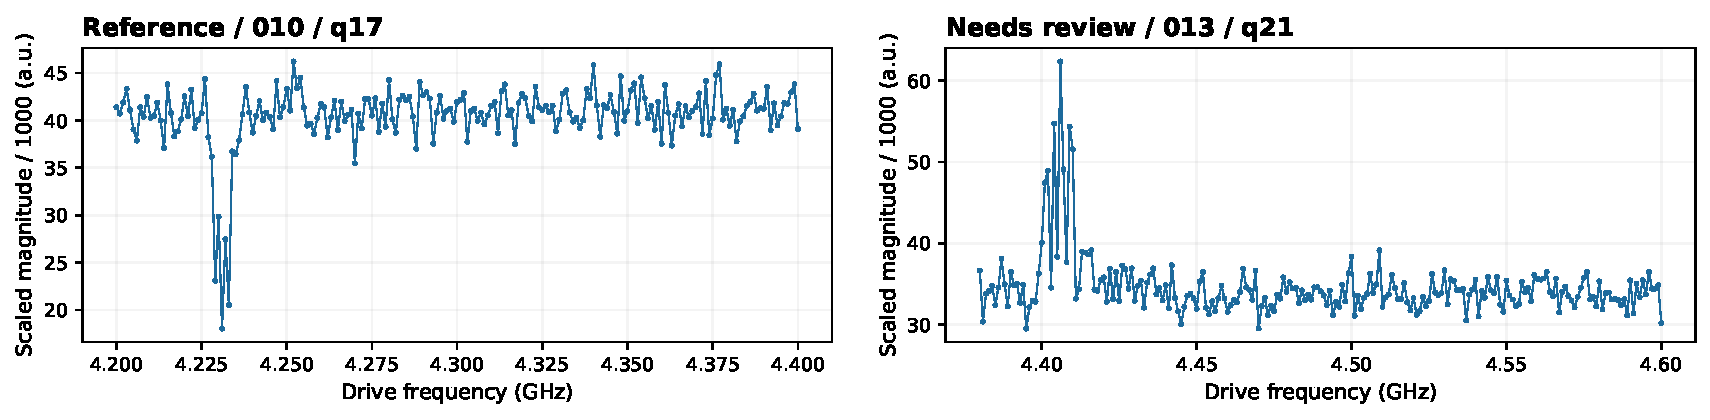
\includegraphics[width=\linewidth,height=34mm,keepaspectratio]{figures/spectroscopy-013.pdf}
\caption{左：对照 010；右：案例 013。IQ 投影诊断： $R^2=0.618$；步长 1.00 / 半高全宽 8.93 MHz。图示幅度；指标来自 IQ 投影的单洛伦兹线形拟合。}
\label{fig-spectroscopy-013}
\end{figure}
\endgroup
{\small\textbf{判断：可见响应不保证单线形模型适用；需细扫并检查线形与背景。}\par}
\end{frame}

\begin{frame}[t,label=case-spectroscopy-014]{背景中的候选响应仍需验证}{Qubit Spectroscopy / 014}
\setlength{\parskip}{0pt}
\begingroup
\setlength{\topsep}{0pt}\setlength{\partopsep}{0pt}
\begin{figure}
\centering
{\small
\makebox[.49\linewidth][c]{\textcolor{Teal}{左：窗口内可见响应与两侧背景}}%
\makebox[.49\linewidth][c]{\textcolor{Orange}{右：背景中的候选响应不够明确}}\par
}
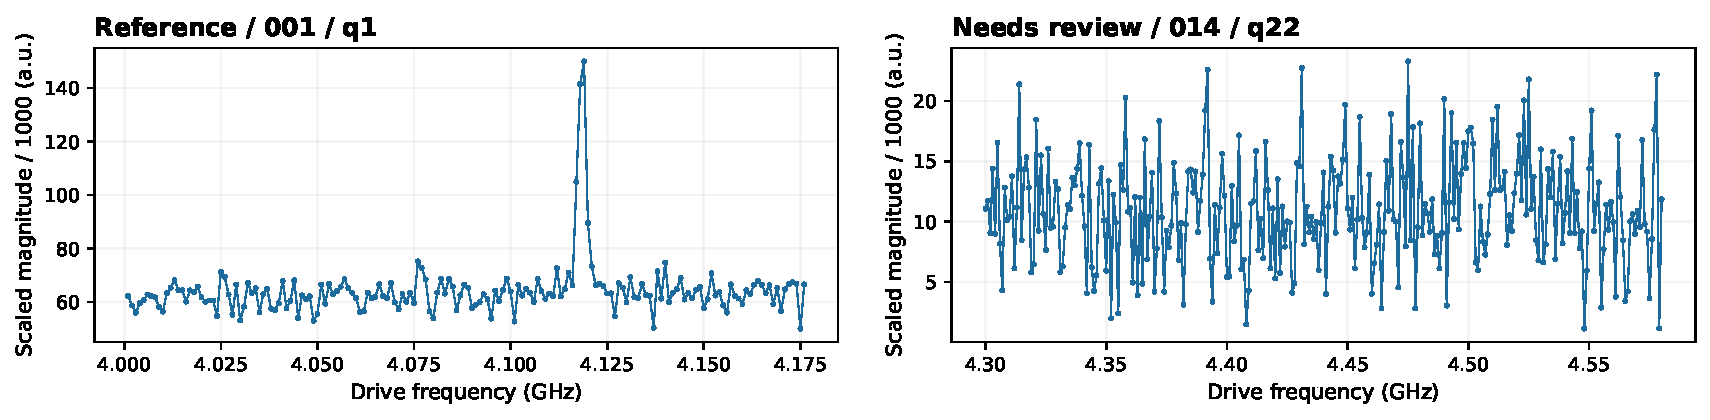
\includegraphics[width=\linewidth,height=34mm,keepaspectratio]{figures/spectroscopy-014.pdf}
\caption{左：对照 001；右：案例 014。IQ 投影诊断： $R^2=0.033$；步长 1.00 / 半高全宽 1.01 MHz。图示幅度；指标来自 IQ 投影的单洛伦兹线形拟合。}
\label{fig-spectroscopy-014}
\end{figure}
\endgroup
{\small\textbf{判断：尚不能确认跃迁频率；需验证信号路径并复测候选响应。}\par}
\end{frame}

\begin{frame}[t,label=case-spectroscopy-015]{背景中的候选响应仍需验证}{Qubit Spectroscopy / 015}
\setlength{\parskip}{0pt}
\begingroup
\setlength{\topsep}{0pt}\setlength{\partopsep}{0pt}
\begin{figure}
\centering
{\small
\makebox[.49\linewidth][c]{\textcolor{Teal}{左：窗口内可见响应与两侧背景}}%
\makebox[.49\linewidth][c]{\textcolor{Orange}{右：背景中的候选响应不够明确}}\par
}
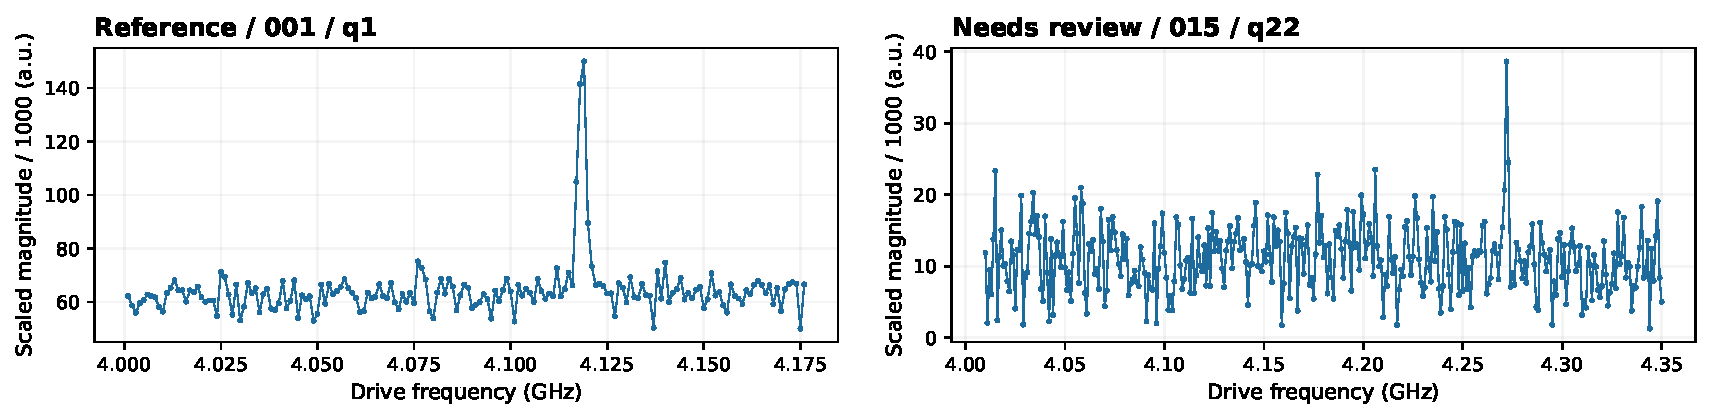
\includegraphics[width=\linewidth,height=34mm,keepaspectratio]{figures/spectroscopy-015.pdf}
\caption{左：对照 001；右：案例 015。IQ 投影诊断： $R^2=0.054$；步长 1.00 / 半高全宽 2.01 MHz。图示幅度；指标来自 IQ 投影的单洛伦兹线形拟合。}
\label{fig-spectroscopy-015}
\end{figure}
\endgroup
{\small\textbf{判断：尚不能确认跃迁频率；需验证信号路径并复测候选响应。}\par}
\end{frame}

\begin{frame}[t,label=case-spectroscopy-016]{可见响应仍需检查线形模型}{Qubit Spectroscopy / 016}
\setlength{\parskip}{0pt}
\begingroup
\setlength{\topsep}{0pt}\setlength{\partopsep}{0pt}
\begin{figure}
\centering
{\small
\makebox[.49\linewidth][c]{\textcolor{Teal}{左：窗口内可见响应与两侧背景}}%
\makebox[.49\linewidth][c]{\textcolor{Orange}{右：单线形拟合仍有未解释结构}}\par
}
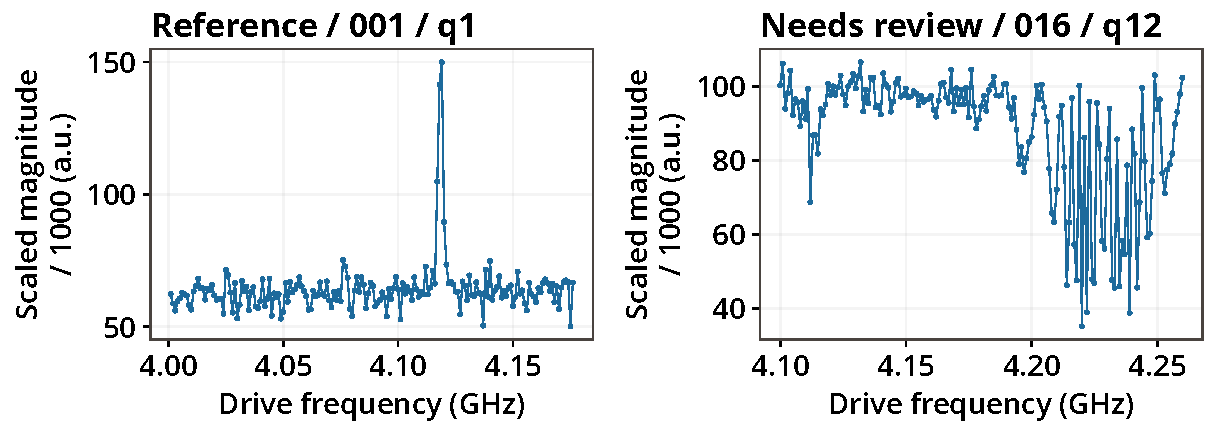
\includegraphics[width=\linewidth,height=34mm,keepaspectratio]{figures/spectroscopy-016.pdf}
\caption{左：对照 001；右：案例 016。IQ 投影诊断： $R^2=0.392$；步长 1.00 / 半高全宽 54.00 MHz。图示幅度；指标来自 IQ 投影的单洛伦兹线形拟合。}
\label{fig-spectroscopy-016}
\end{figure}
\endgroup
{\small\textbf{判断：可见响应不保证单线形模型适用；需细扫并检查线形与背景。}\par}
\end{frame}

\begin{frame}[t,label=case-spectroscopy-017]{可见响应仍需检查线形模型}{Qubit Spectroscopy / 017}
\setlength{\parskip}{0pt}
\begingroup
\setlength{\topsep}{0pt}\setlength{\partopsep}{0pt}
\begin{figure}
\centering
{\small
\makebox[.49\linewidth][c]{\textcolor{Teal}{左：窗口内可见响应与两侧背景}}%
\makebox[.49\linewidth][c]{\textcolor{Orange}{右：单线形拟合仍有未解释结构}}\par
}
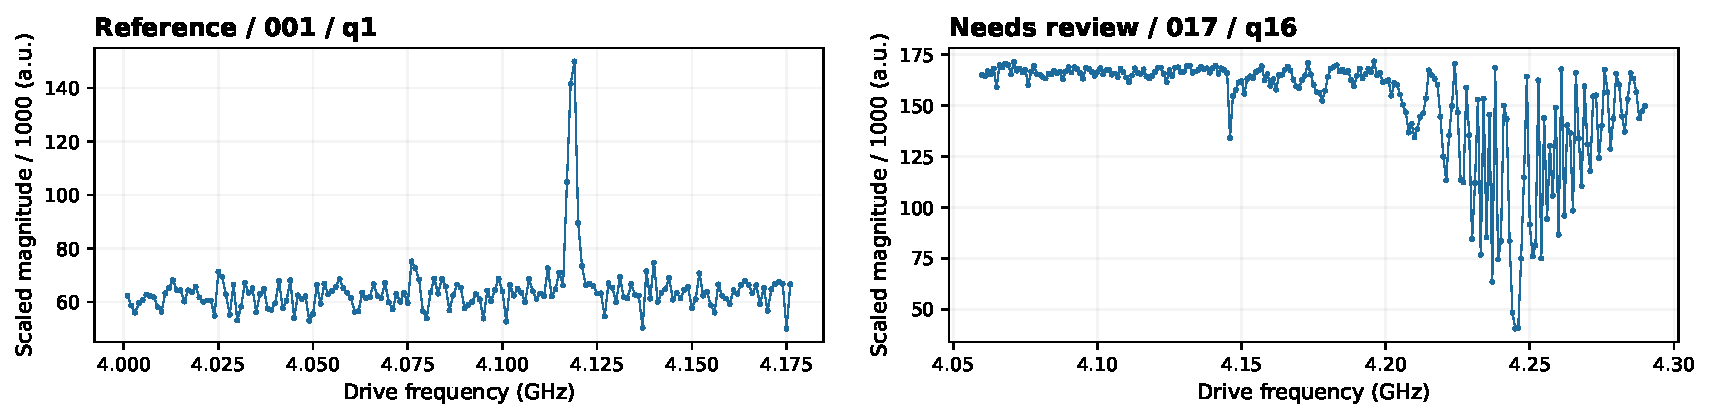
\includegraphics[width=\linewidth,height=34mm,keepaspectratio]{figures/spectroscopy-017.pdf}
\caption{左：对照 001；右：案例 017。IQ 投影诊断： $R^2=0.619$；步长 1.00 / 半高全宽 30.87 MHz。图示幅度；指标来自 IQ 投影的单洛伦兹线形拟合。}
\label{fig-spectroscopy-017}
\end{figure}
\endgroup
{\small\textbf{判断：可见响应不保证单线形模型适用；需细扫并检查线形与背景。}\par}
\end{frame}

\begin{frame}[t,label=case-spectroscopy-018]{频率步长不能分辨拟合线宽}{Qubit Spectroscopy / 018}
\setlength{\parskip}{0pt}
\begingroup
\setlength{\topsep}{0pt}\setlength{\partopsep}{0pt}
\begin{figure}
\centering
{\small
\makebox[.49\linewidth][c]{\textcolor{Teal}{左：窗口内可见响应与两侧背景}}%
\makebox[.49\linewidth][c]{\textcolor{Orange}{右：候选线宽内采样点不足}}\par
}
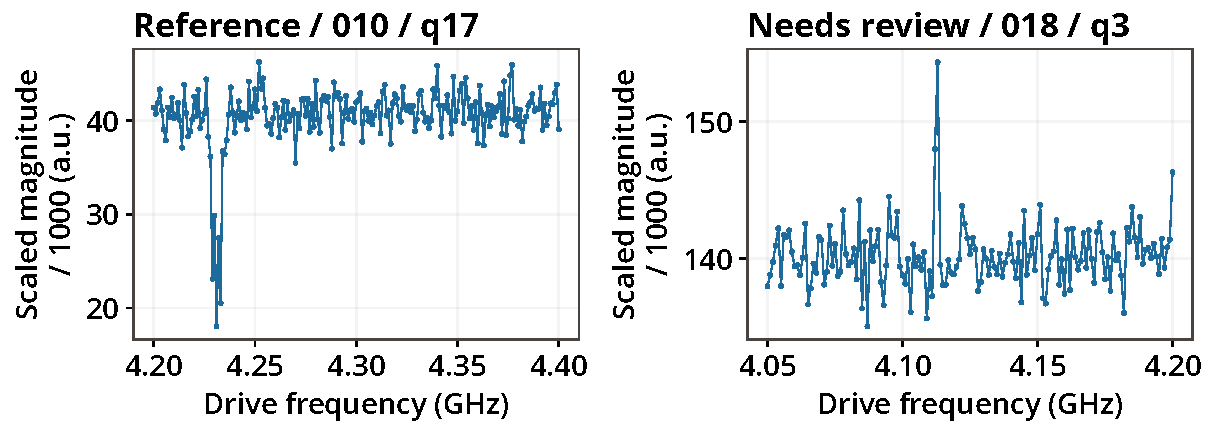
\includegraphics[width=\linewidth,height=34mm,keepaspectratio]{figures/spectroscopy-018.pdf}
\caption{左：对照 010；右：案例 018。IQ 投影诊断： $R^2=0.929$；步长 1.00 / 半高全宽 1.05 MHz。图示幅度；指标来自 IQ 投影的单洛伦兹线形拟合。}
\label{fig-spectroscopy-018}
\end{figure}
\endgroup
{\small\textbf{判断：线宽缺乏采样约束；需局部细扫并复测。}\par}
\end{frame}

\begin{frame}[t,label=case-readout-002]{两组准备条件的区分仍需验证}{GMM Readout Clusters / 002}
\setlength{\parskip}{0pt}
\begingroup
\setlength{\topsep}{0pt}\setlength{\partopsep}{0pt}
\begin{figure}
\centering
{\small
\makebox[.49\linewidth][c]{\textcolor{Teal}{左：准备条件较易区分}}%
\makebox[.49\linewidth][c]{\textcolor{Orange}{右：准备条件的分布仍有重叠}}\par
}
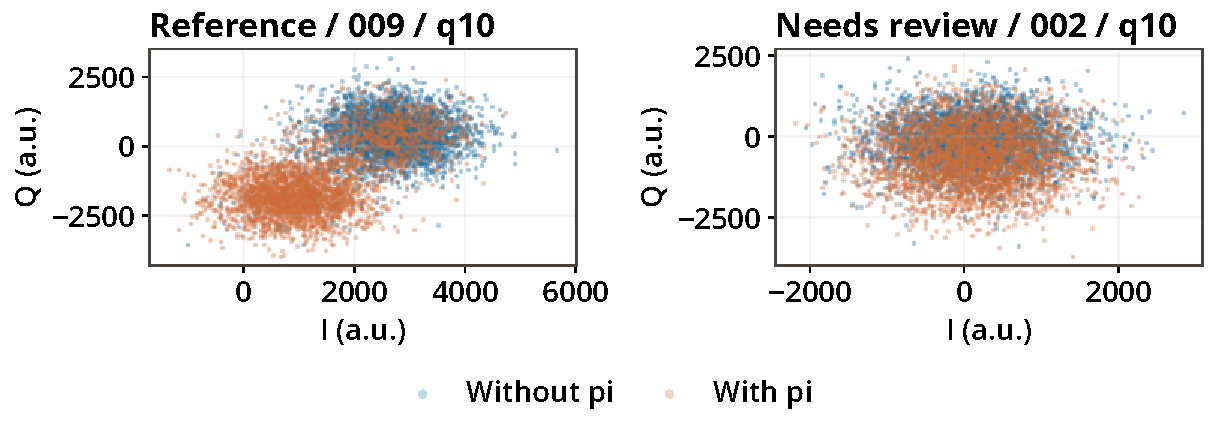
\includegraphics[width=\linewidth,height=34mm,keepaspectratio]{figures/readout-002.pdf}
\caption{左：对照 009；右：案例 002。线性分类器的留出评估平衡准确率： $62.12\%$。预测准备标签；包含状态准备与弛豫的影响。}
\label{fig-readout-002}
\end{figure}
\endgroup
{\small\textbf{判断：区分程度不足；需分别验证准备与读出，不能单独归因于测量。}\par}
\end{frame}

\begin{frame}[t,label=case-readout-003]{两组准备条件的区分仍需验证}{GMM Readout Clusters / 003}
\setlength{\parskip}{0pt}
\begingroup
\setlength{\topsep}{0pt}\setlength{\partopsep}{0pt}
\begin{figure}
\centering
{\small
\makebox[.49\linewidth][c]{\textcolor{Teal}{左：准备条件较易区分}}%
\makebox[.49\linewidth][c]{\textcolor{Orange}{右：准备条件的分布仍有重叠}}\par
}
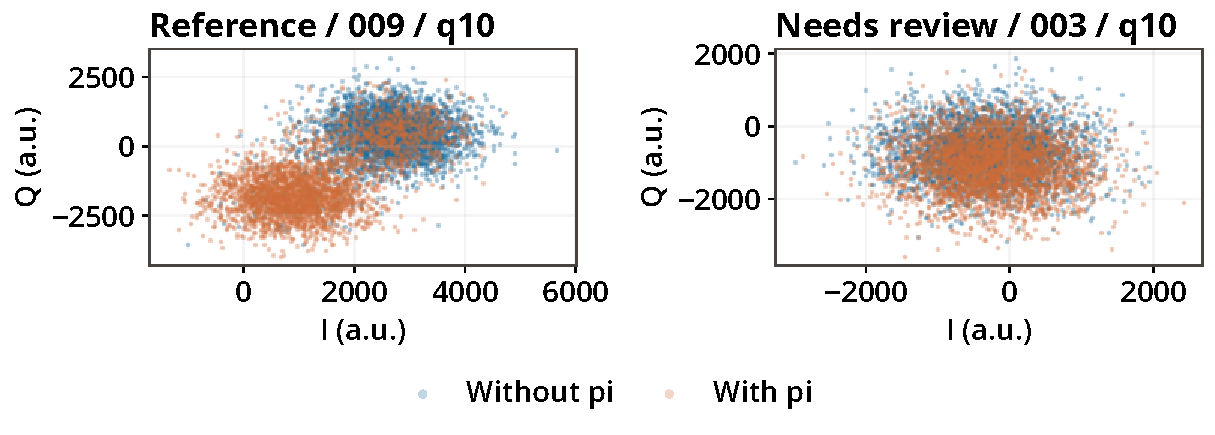
\includegraphics[width=\linewidth,height=34mm,keepaspectratio]{figures/readout-003.pdf}
\caption{左：对照 009；右：案例 003。线性分类器的留出评估平衡准确率： $59.67\%$。预测准备标签；包含状态准备与弛豫的影响。}
\label{fig-readout-003}
\end{figure}
\endgroup
{\small\textbf{判断：区分程度不足；需分别验证准备与读出，不能单独归因于测量。}\par}
\end{frame}

\begin{frame}[t,label=case-readout-004]{两组准备条件的区分仍需验证}{GMM Readout Clusters / 004}
\setlength{\parskip}{0pt}
\begingroup
\setlength{\topsep}{0pt}\setlength{\partopsep}{0pt}
\begin{figure}
\centering
{\small
\makebox[.49\linewidth][c]{\textcolor{Teal}{左：准备条件较易区分}}%
\makebox[.49\linewidth][c]{\textcolor{Orange}{右：准备条件的分布仍有重叠}}\par
}
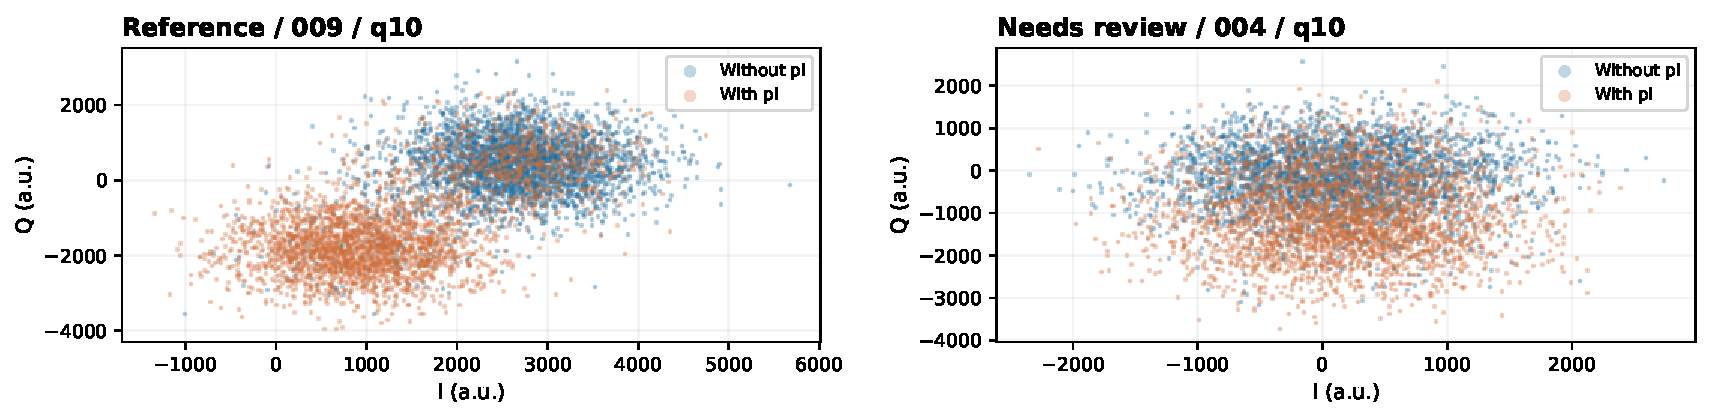
\includegraphics[width=\linewidth,height=34mm,keepaspectratio]{figures/readout-004.pdf}
\caption{左：对照 009；右：案例 004。线性分类器的留出评估平衡准确率： $70.73\%$。预测准备标签；包含状态准备与弛豫的影响。}
\label{fig-readout-004}
\end{figure}
\endgroup
{\small\textbf{判断：区分程度不足；需分别验证准备与读出，不能单独归因于测量。}\par}
\end{frame}

\begin{frame}[t,label=case-readout-005]{接近筛查阈值仍需结合数据判断}{GMM Readout Clusters / 005}
\setlength{\parskip}{0pt}
\begingroup
\setlength{\topsep}{0pt}\setlength{\partopsep}{0pt}
\begin{figure}
\centering
{\small
\makebox[.49\linewidth][c]{\textcolor{Teal}{左：准备条件较易区分}}%
\makebox[.49\linewidth][c]{\textcolor{Orange}{右：准确率略低于本地筛查阈值}}\par
}
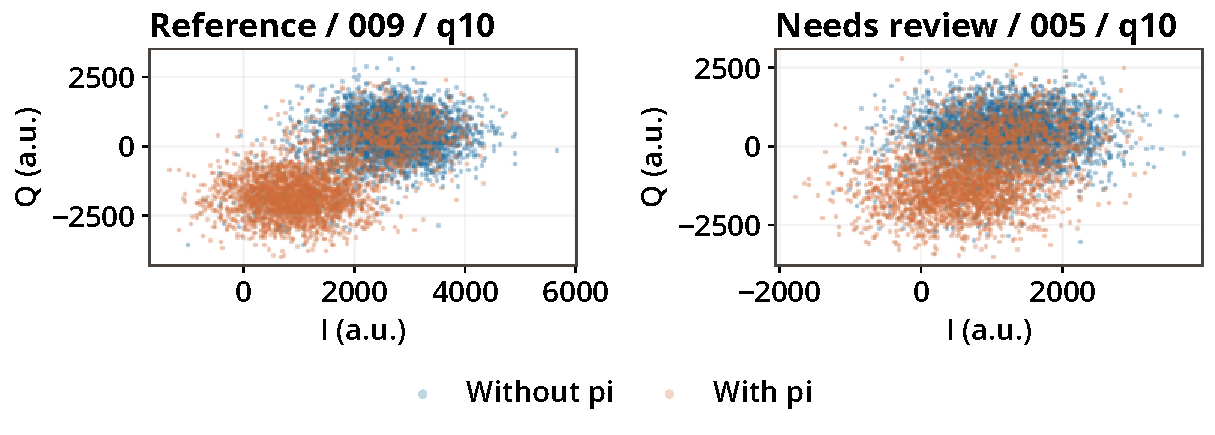
\includegraphics[width=\linewidth,height=34mm,keepaspectratio]{figures/readout-005.pdf}
\caption{左：对照 009；右：案例 005。线性分类器的留出评估平衡准确率： $74.48\%$。预测准备标签；包含状态准备与弛豫的影响。}
\label{fig-readout-005}
\end{figure}
\endgroup
{\small\textbf{判断：需结合重复测量判断；筛查阈值本身不构成物理失败标准。}\par}
\end{frame}
